\documentclass[aspectratio=10]{beamer} %For normal presentation (comment otherwise)
%\documentclass[aspectratio=169]{beamer} %for widescreen prestentation
\usetheme{Marburg}
\usefonttheme{serif}
\usecolortheme{default}%albatross, crane, beetle, dove, fly, seagull, wolverine e beaver.
%%%%%%%%%%%%%%%%%%%%%%%%%%%%%%%%%%%%%%%%%%%%%%%%%%%%%%%%%%%%%%%%%%%%%%%%%%%%%%%%%%%%%%%%%%%%%%%
%%%%%%%%%%%%%%%%%%%%%%%%%%%%%%%%%%%%%%EXTRA PACTAGES%%%%%%%%%%%%%%%%%%%%%%%%%%%%%%%%%%%%%%%%%%%
\usepackage[utf8]{inputenc}
\usepackage[T1]{fontenc}
\usepackage[portuguese, english]{babel}
\usepackage[round]{natbib}
\usepackage{hyperref} 
\usepackage{graphicx} % Required for including images
\usepackage{graphics}
\graphicspath{{Imagens/}} % Location of the graphics files
\usepackage{booktabs} % Top and bottom rules for table
\usepackage[font=small,labelfont=bf]{caption}%specifies captions on tables and figures
\usepackage{amsfonts, amsmath, amsthm, amssymb} % For math fonts, symbols and environments
\usepackage{wrapfig} % Allows wrapping text around tables and figures
\usepackage{makeidx}
\usepackage{lipsum} % Required to insert dummy text. To be removed otherwise
\usepackage{epstopdf}%adiciona imagens em formato eps no pdf.
\usepackage{subfigure}%cria ambientes de multifiguras
\usepackage{float}%coloca as figuras exatamente aonde você quer
\usepackage{times}
\usepackage{tikz}%pacote para fazer fluxogramas
\usepackage{verbatim}%
\usepackage{smartdiagram}
%%%%%%%%%%%%%%%%%%%%%%%%%%%%%%%%%%%%%%%%%%%%%%%%%%%%%%%%%%%%%%%%%%%%%%%%%%%%%%%%%%%%%%%%%%%%%
%%%%%%%%%%%%%%%%%%%%%%%%%%%%%%%%%%%%%PREAMBLE%%%%%%%%%%%%%%%%%%%%%%%%%%%%%%%%%%%%%%%%%%%%%%%%
\author[Carreira,V.R.]{Authors: Victor Ribeiro Carreira$^{1}$, Cosme Ferreira Ponte Neto$^{1}$, Rodrigo Bijani Santos$^{1}$}
\title{A Comparison of Machine Learning Processes for Classification of Rock Units Using Well Log Data}
%\subtitle{}
\institute{Observatório Nacional$^{1}$}
\date{June 2018}
\subject{EAGE  ANNUAL 80TH CONFERENCE + EXHIBITION. COPENHAGEN, DENMARK. 2018}
%\setbeamertemplate{footline}[frame number]
%\setbeamercovered{transparent}
%\setbeamertemplate{navigation symbols}{}
% Tela cheia
\hypersetup{pdfpagemode=FullScreen}
\usepackage{ragged2e}
\justifying
\addtobeamertemplate{headline}{} 
{\begin{tikzpicture}[remember picture, overlay]
	\node [anchor=south west, inner sep=0.4cm]  at (current page.south west)
	{
\includegraphics[height=0.4cm]{Imagens/eage18.eps}};
	\end{tikzpicture}}
%%%%%%%%%%%%%%%%%%%%%%%%%%%%%%%%%%%%%%%%%%%%%%%%%%%%%%%%%%%%%%%%%%%%%%%%%%%%%%%%%%%%%%%%%%%%%%%%%%%%%%%%%%%%%%%%%%%%%%%%%%%%%%%%%%%%%%PRESENTATION%%%%%%%%%%%%%%%%%%%%%%%%%%%%%%%%%%%%%%%%%%%%%%%%%%%%%%%%%%%%%%%%%%%%%%%%%%%%%%%%%%%%%%%%%%%%%%%%%%%%%%%%%%%%%%%%%%%%%%%%%%%%%%%%%%%%%%%%%%%
\begin{document}

	\bgroup
	\makeatletter
	\setbeamertemplate{footline}
	\makeatother

%\maketitle
\egroup 
\addtobeamertemplate{navigation symbols}{}{\hskip6pt\raisebox{2pt}{\color{blue}\insertframenumber}}
\setcounter{framenumber}{-1}
\AtBeginSection[]


\begin{frame}
 \flushbottom
 \setlength{\parskip}{-1ex plus 1ex }
 \setlength{\parindent}{-15pt}
 
\includegraphics[width=13cm,height=10cm]{Imagens/front.pdf}
\end{frame}


\section{Introduction}

\subsection{Motivation}


{%
	\usebackgroundtemplate{
		\centering
		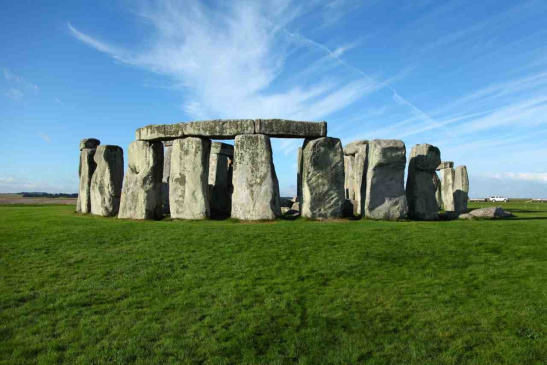
\includegraphics[width=\paperwidth,height=\paperheight]{Imagens/stonerange.jpg}
	}
	
	% Frame 3: plano de fundo
	\begin{frame}
	\frametitle{\textcolor{yellow}{Changing seasons}}
	%\flushbottom\color{yellow}{\normalsize Changing seasons}
	
\end{frame}
}

{%
\usebackgroundtemplate{
	\centering
	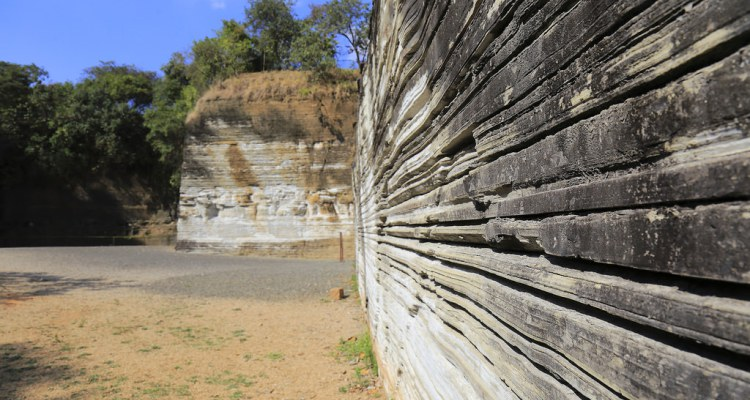
\includegraphics[width=\paperwidth,height=\paperheight]{Imagens/varvite.jpg}
}

% Frame 3: plano de fundo
\begin{frame}
\frametitle{\textcolor{yellow}{Varvite (Itu - São Paulo)}}
%\flushbottom\color{yellow}{\normalsize Changing seasons}

\end{frame}
}


\begin{frame}
\frametitle{Introduction}

\begin{itemize}
	\item Machine learning approaches computer program's that have the capability of automatically improve themselves through experience \citep{Michie1994, Levy1997, MacKay2005}.
	\pause
	\item Classification techniques uses distances attributes \citep{Michel2016}.
	\pause
	\item Euclidean classifier calculates a centroid in the space of attributes.
	\pause
	\item Mahalanobis classifier takes into consideration the shape of attributes space.
	\pause
	\item A Self Organizing Map (SOM) is inspired by neural cortex \citep{Kohonen1989} and based oriented graph \citep{Haykin1999} working as an interconnected network. 
	
\end{itemize}

\end{frame}

\subsection{Objective}

\begin{frame}
\frametitle{Objective}
	\begin{itemize}
		\item Define comparisons between a Kohonen (SOM), an euclidean and a mahalanobean classifiers.
		\pause
		\item Using synthetic well log data in a controlled situation.
	\end{itemize}
\end{frame}


\section{Methodology}

\subsection{Synthetic Sedimentary Basin}




\begin{frame}
	\frametitle{Methodology}
	\smartdiagram[priority descriptive diagram]{
		Generates the hypothesis model,
	    Uses T1 well data to train the Kohonen (SOM) and make the statistical of classifiers,
		Uses C1 and C2 to make predictions using SOM and the classifiers,
		Compare the results					}
\end{frame}


\begin{frame}
	\frametitle{Synthetic Sedimentary Basin}
	\begin{figure}[H]
		\centering
		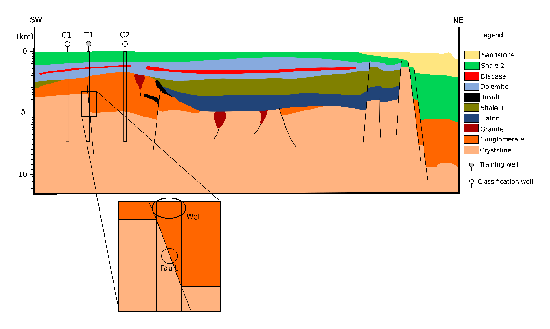
\includegraphics[scale=0.34]{Imagens/Basin.eps}
		\caption{Synthetic Sedimentary Basin by \cite{Sal2008}  T1, C1 and C2 are training and classifing wells respectively.}
		\label{Model}
	\end{figure}
\end{frame}


\begin{frame}
\frametitle{Synthetic Sedimentary Basin}
\begin{table}[H]\tiny
	\caption{Physical properties and rock types.}
\begin{tabular}{@{}ccccccccccc@{}}
	\toprule
	Rock & Density ($g/cm^{3}$) & Gamma ray ($Ci/g$) & Resistivity ($\Omega.m$)& Velocity ($Km/s$) &\\ \midrule
	Conglomerate &     $2.30$ 		  &       $100.0$       &           $6000$           &			$2$   		   	&\\
	Shale	 &       $2.55$           &       $100.0$       &           $1000$           &     		$3$		 &\\
	Dolomite     &       $2.72$           &       $8.30$        &           $3.5 \times 10^{3}$           &  	$6$    			 &\\
	Diabase    &       $2.91$           &       $30.0$        &           $15 \times 10^{7}$           &      $5.5$				 &\\
	Crystalline  &       $2.80$           &       $0.7$         &           $1.3 \times 10^{6}$           & 		$5$		     &\\ \bottomrule
\end{tabular}

\label{Tab1}
\end{table}

\begin{itemize}\footnotesize
	\item  The sample rate for the well data is $0.01$ observation/meter with contamination of $5$\% Gaussian noise.
\end{itemize}
\end{frame}

\subsection{Training and Similarities}

\begin{frame}
	\frametitle{Training and Similarities}
	\begin{figure}[H]
		\centering
		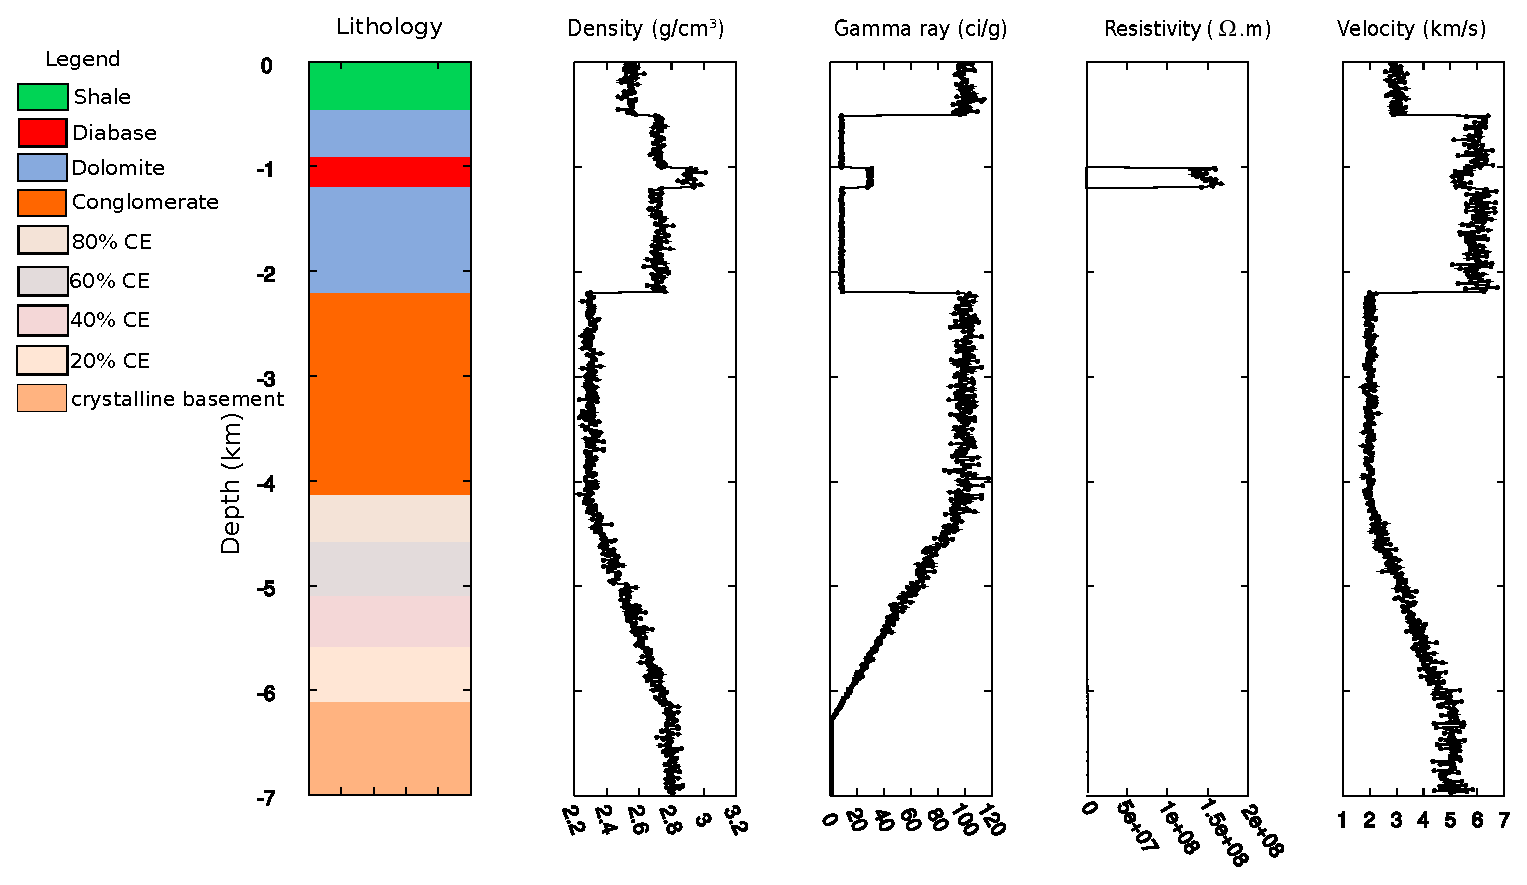
\includegraphics[scale=0.34]{Imagens/Pocot1.eps}
		\caption{Synthetic training well T$1$.}
		\label{T1}
	\end{figure}
\pause
\begin{itemize}\footnotesize
	\item Four divisions describes the normal fault by decreasing the amount of conglomerate in comparison to crystalline basement.
\end{itemize}

\end{frame}

\begin{frame}
\frametitle{Training and Similarities}
\begin{figure}[H]
	\centering
	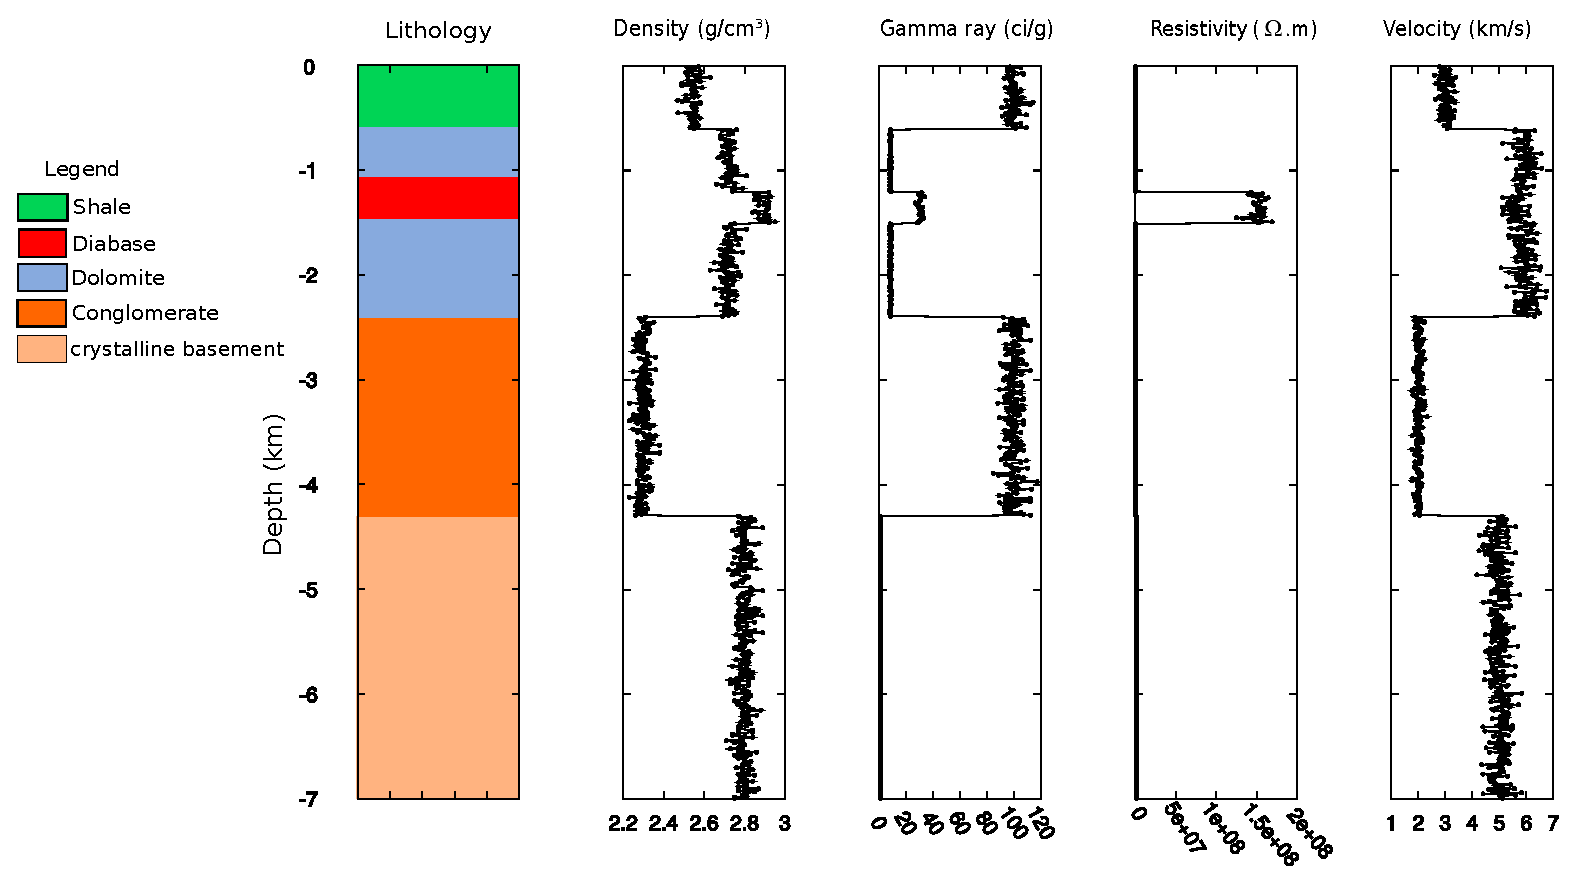
\includegraphics[scale=0.39]{Imagens/Pococ1.eps}
	\caption{Classification well C$1$}
	\label{C1}
\end{figure}
\end{frame}

\begin{frame}
\frametitle{Training and Similarities}
\begin{figure}[H]
	\centering
	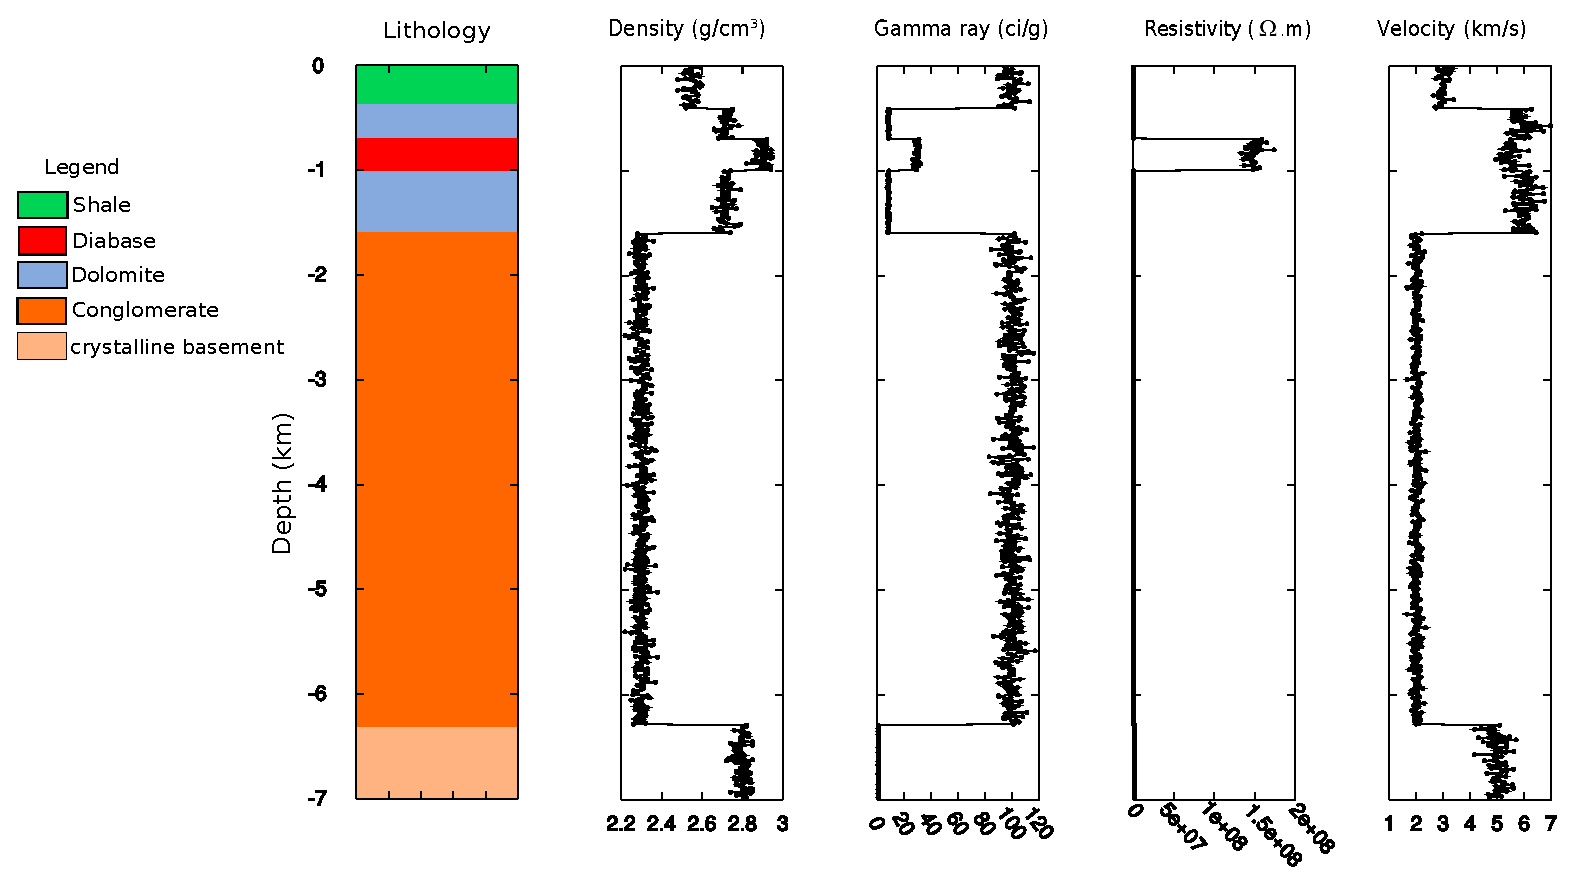
\includegraphics[scale=0.39]{Imagens/Pococ2.eps}
	\caption{Classification well C$2$}
	\label{C2}
\end{figure}
\end{frame}



\subsubsection{Euclidean Classifier}

\begin{frame}
	\frametitle{Euclidean Classifier}
	
	\begin{equation}
	Ed_{i} =  \Arrowvert \textbf{X}-\bar{\textbf{X}}_{i}  \Arrowvert^{\frac{1}{2}}, 
	\label{eq4}
	\end{equation}  
	 \pause
	\begin{itemize}
		\centering
		\item[$\textbf{X}$], input vector 
		\pause
		\item[$\bar{\textbf{X}}_{i}$], mean vector
	\end{itemize}
	
\end{frame}
  

\begin{frame}
  \frametitle{Euclidean Classifier}
  
    \begin{figure}[H]
    	
    	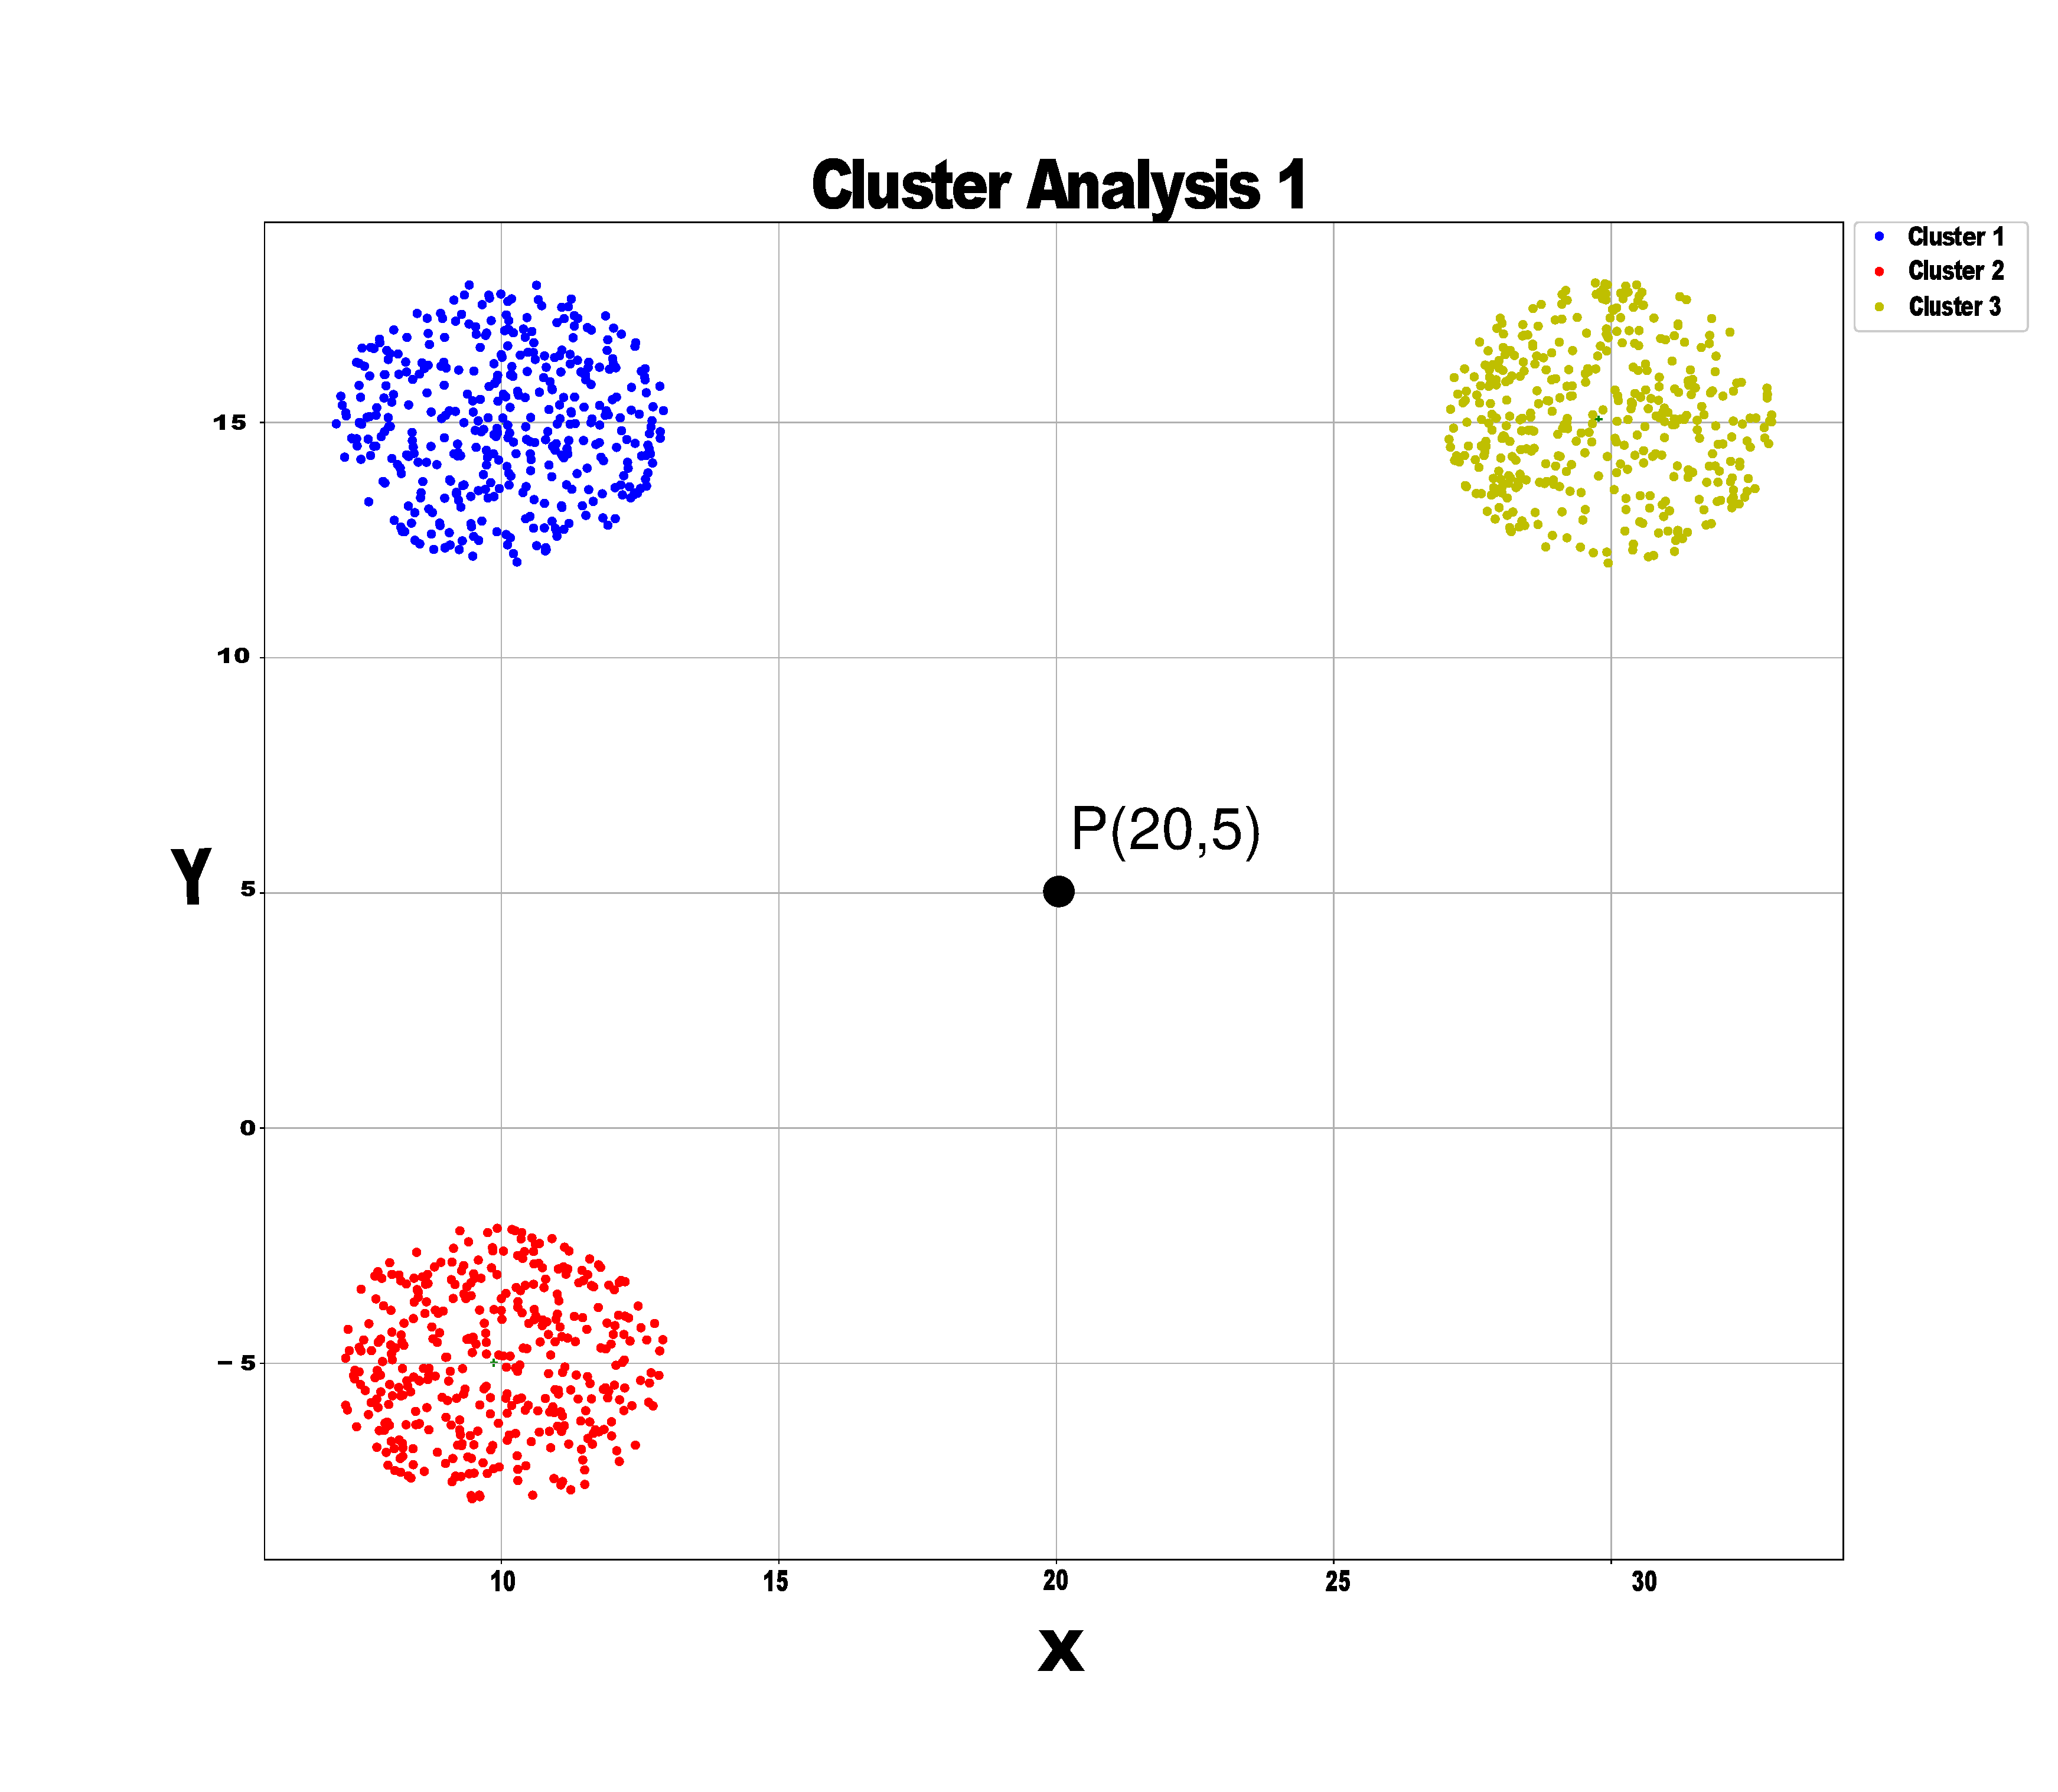
\includegraphics[scale=0.13]{Imagens/clusteranalise1.eps}
    \end{figure}
  
\end{frame}

\begin{frame}
\frametitle{Euclidean Classifier}

\begin{figure}[H]
	
	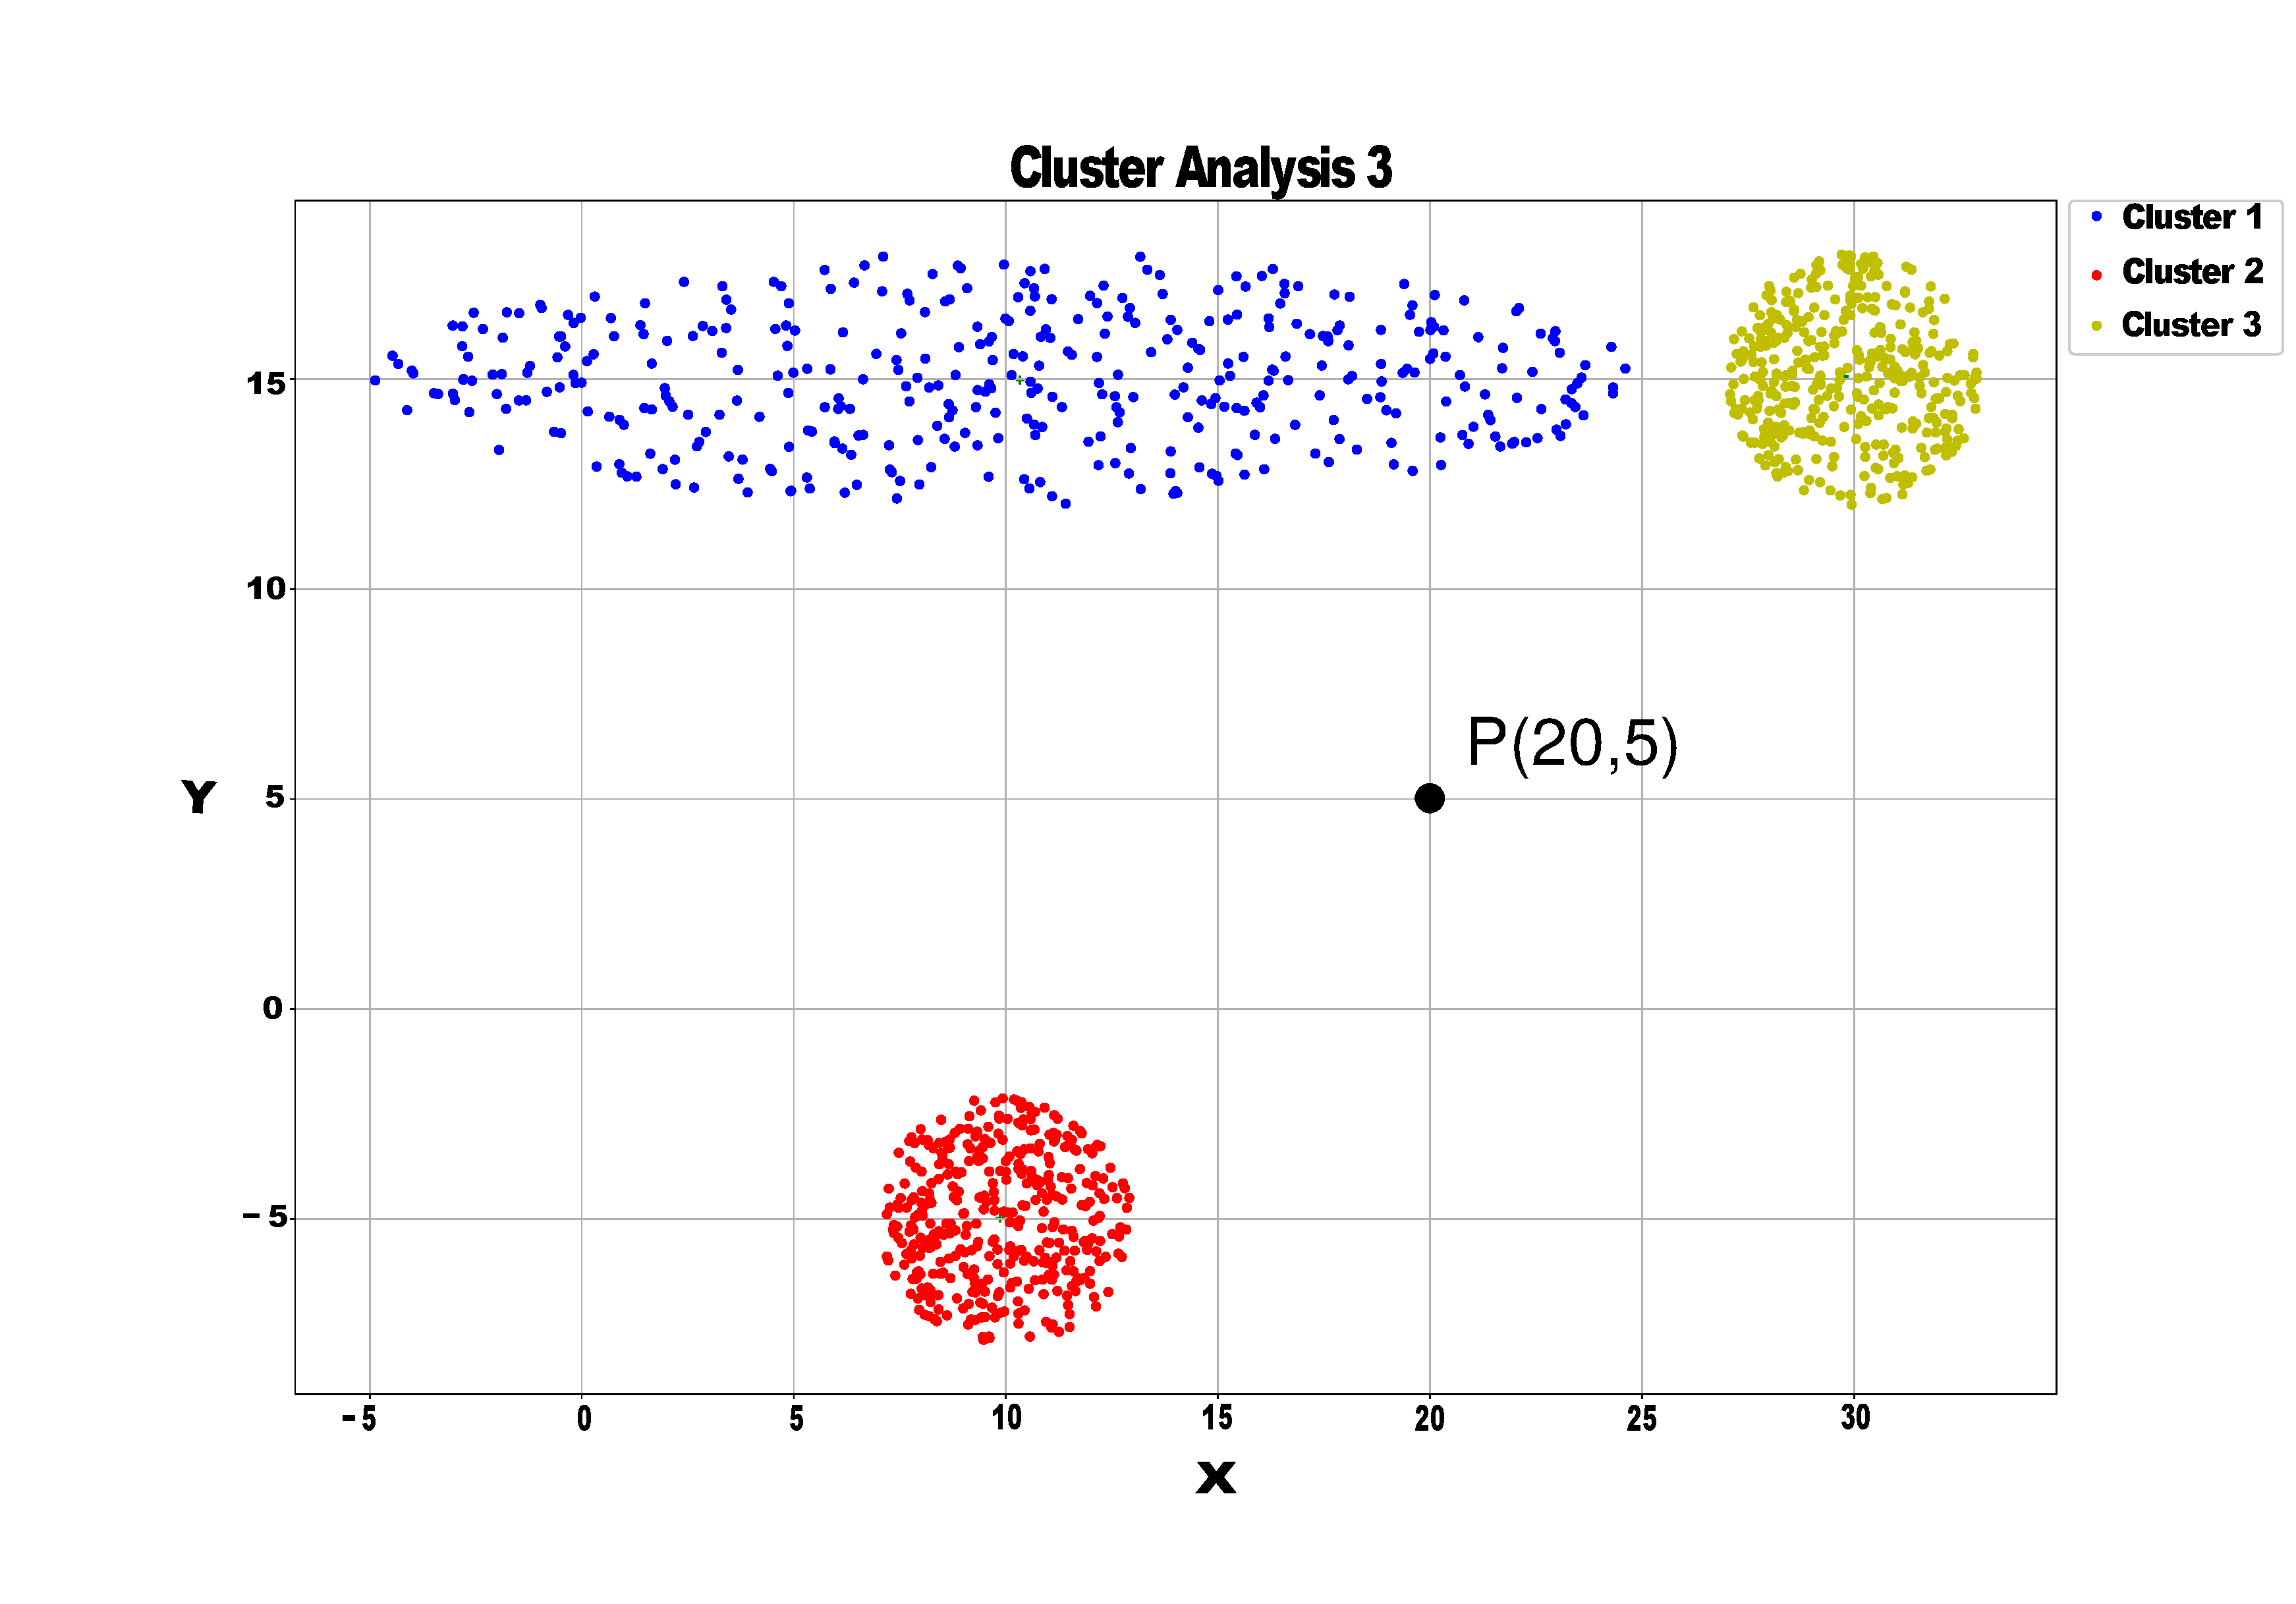
\includegraphics[scale=0.13]{Imagens/clusteranalise3.eps}
\end{figure}

\end{frame}

\subsubsection{Mahalanobis Classifier}

\begin{frame}
	\frametitle{Mahalanobis Classifier}
	
	\begin{equation}
	Md_{i}=[(\textbf{X}-\bar{\textbf{X}}_{i})^{T}\textbf{C}_{i}^{-1}(\textbf{X}-\bar{\textbf{X}}_{i})]^{\frac{1}{2}}.
	\label{eq5}
	\end{equation}
	 \pause
	\begin{itemize}
		\centering
    	\item[$\textbf{X}$], input vector 
		\pause
		\item[$\bar{\textbf{X}}_{i}$], mean vector
		\pause
		\item[$\textbf{C}_{i}$], covariance matrix
	\end{itemize}
\end{frame}


\begin{frame}
\frametitle{Mahalanobis Classifier}

\begin{equation}
\textbf{C}_{i}=\frac{1}{n_{i}-1}\sum_{X \in \omega_{i}}(\textbf{X}-\bar{\textbf{X}}_{i})(\textbf{X}-\bar{\textbf{X}}_{i})^{T}
\label{eq6}
\end{equation}
\pause
\begin{itemize}
	\centering
	\item[$n_{i}$], number of elements  
	\pause
	\item[$\omega_{i}$], space of attributes
\end{itemize}
\end{frame}

\subsubsection{Clusters and Space of Attributes}

\begin{frame}
	\frametitle{Clusters and Space of Attributes - T1 well}
	    
	\begin{figure}
	 %\centering
	 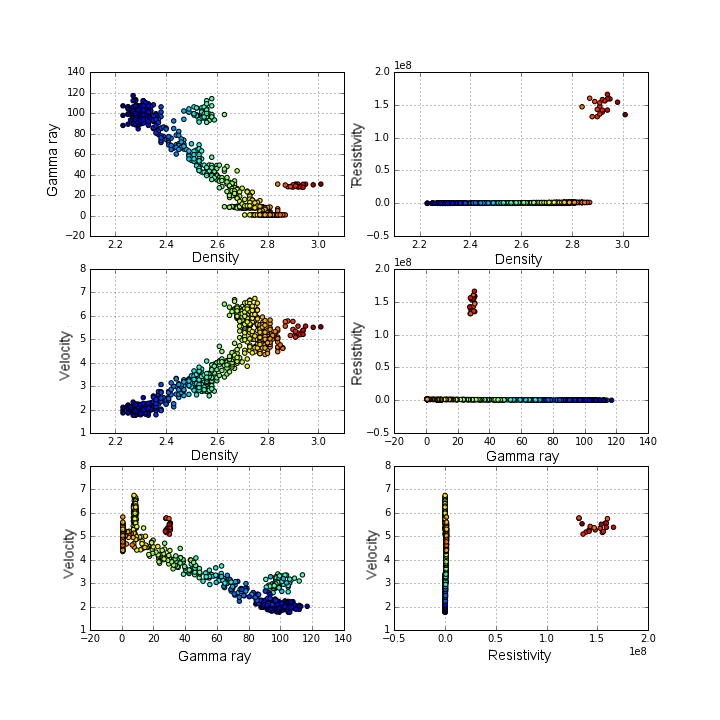
\includegraphics[scale=0.29]{Imagens/cluterpocoT1.png}
	\end{figure}
	
\end{frame}


\begin{frame}
\frametitle{Clusters and Space of Attributes - C1 well}

\begin{figure}
	%\centering
	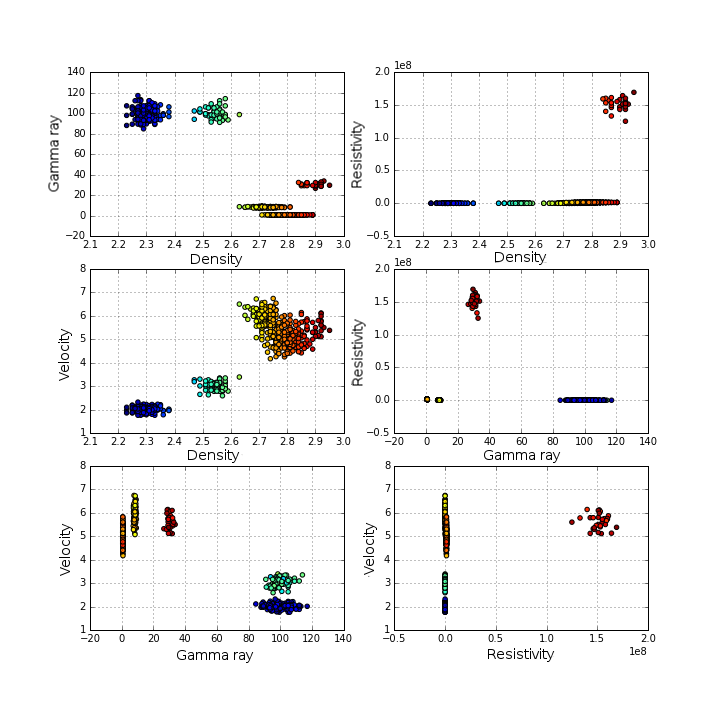
\includegraphics[scale=0.29]{Imagens/cluterpocoC1.png}
\end{figure}

\end{frame}

\begin{frame}
\frametitle{Clusters and Space of Attributes - C2 well}

\begin{figure}
	%\centering
	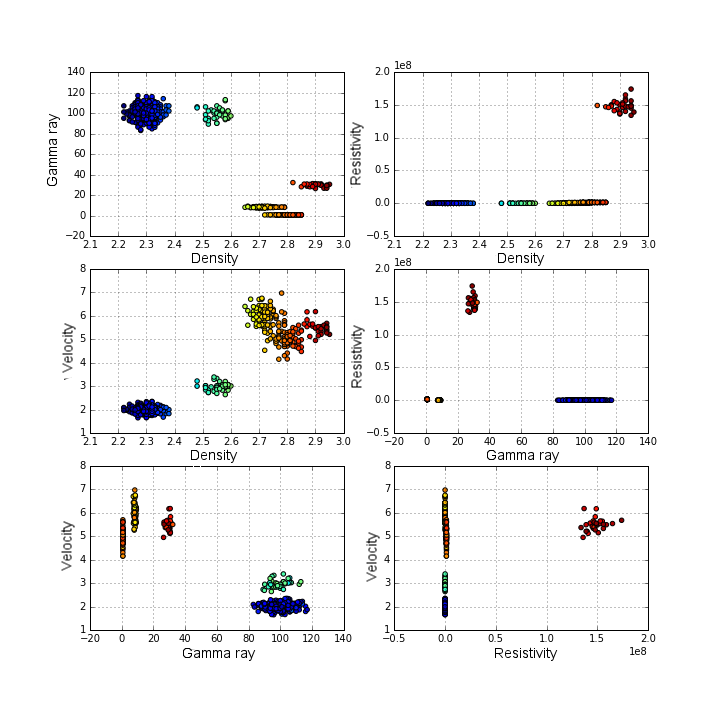
\includegraphics[scale=0.29]{Imagens/cluterpocoC2.png}
\end{figure}

\end{frame}

\subsubsection{Kohonen - SOM}


\begin{frame}
  \frametitle{Kohonen - SOM}
  	 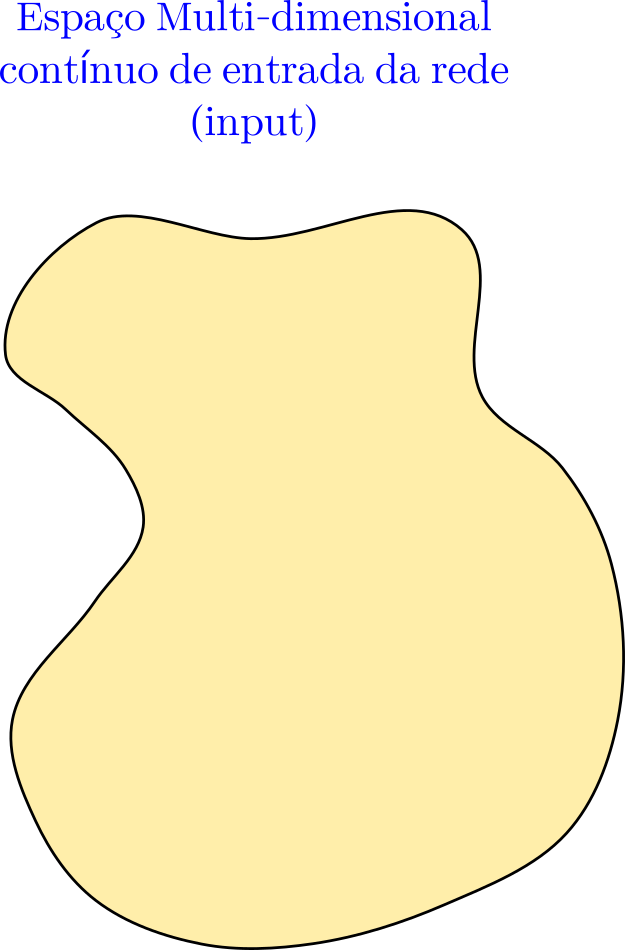
\includegraphics[scale=0.5]{Imagens/IntroKoho1.png} 
\end{frame}


\begin{frame}
 \frametitle{Kohonen - SOM}
 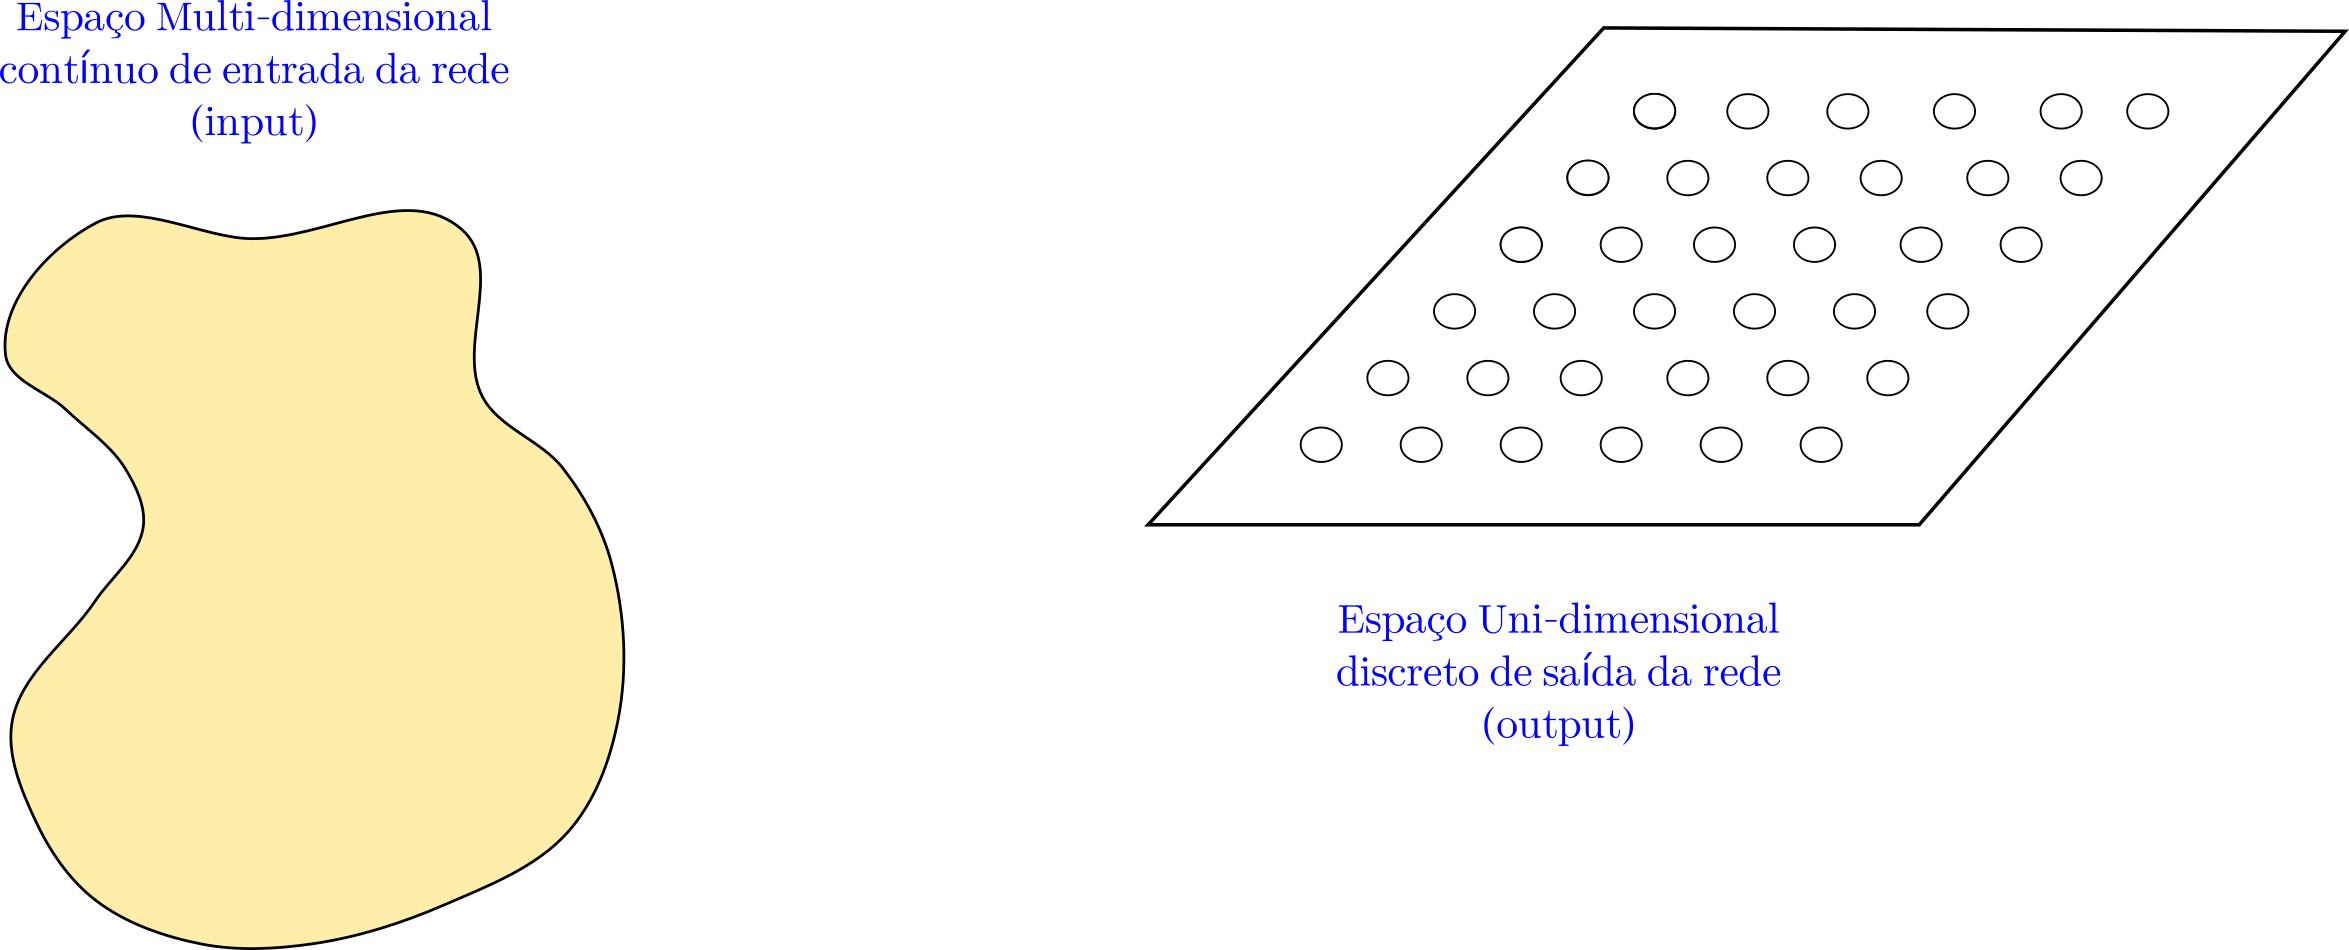
\includegraphics[scale=0.5]{Imagens/IntroKoho2.png} 
\end{frame}


\begin{frame}
 \frametitle{Kohonen - SOM}
 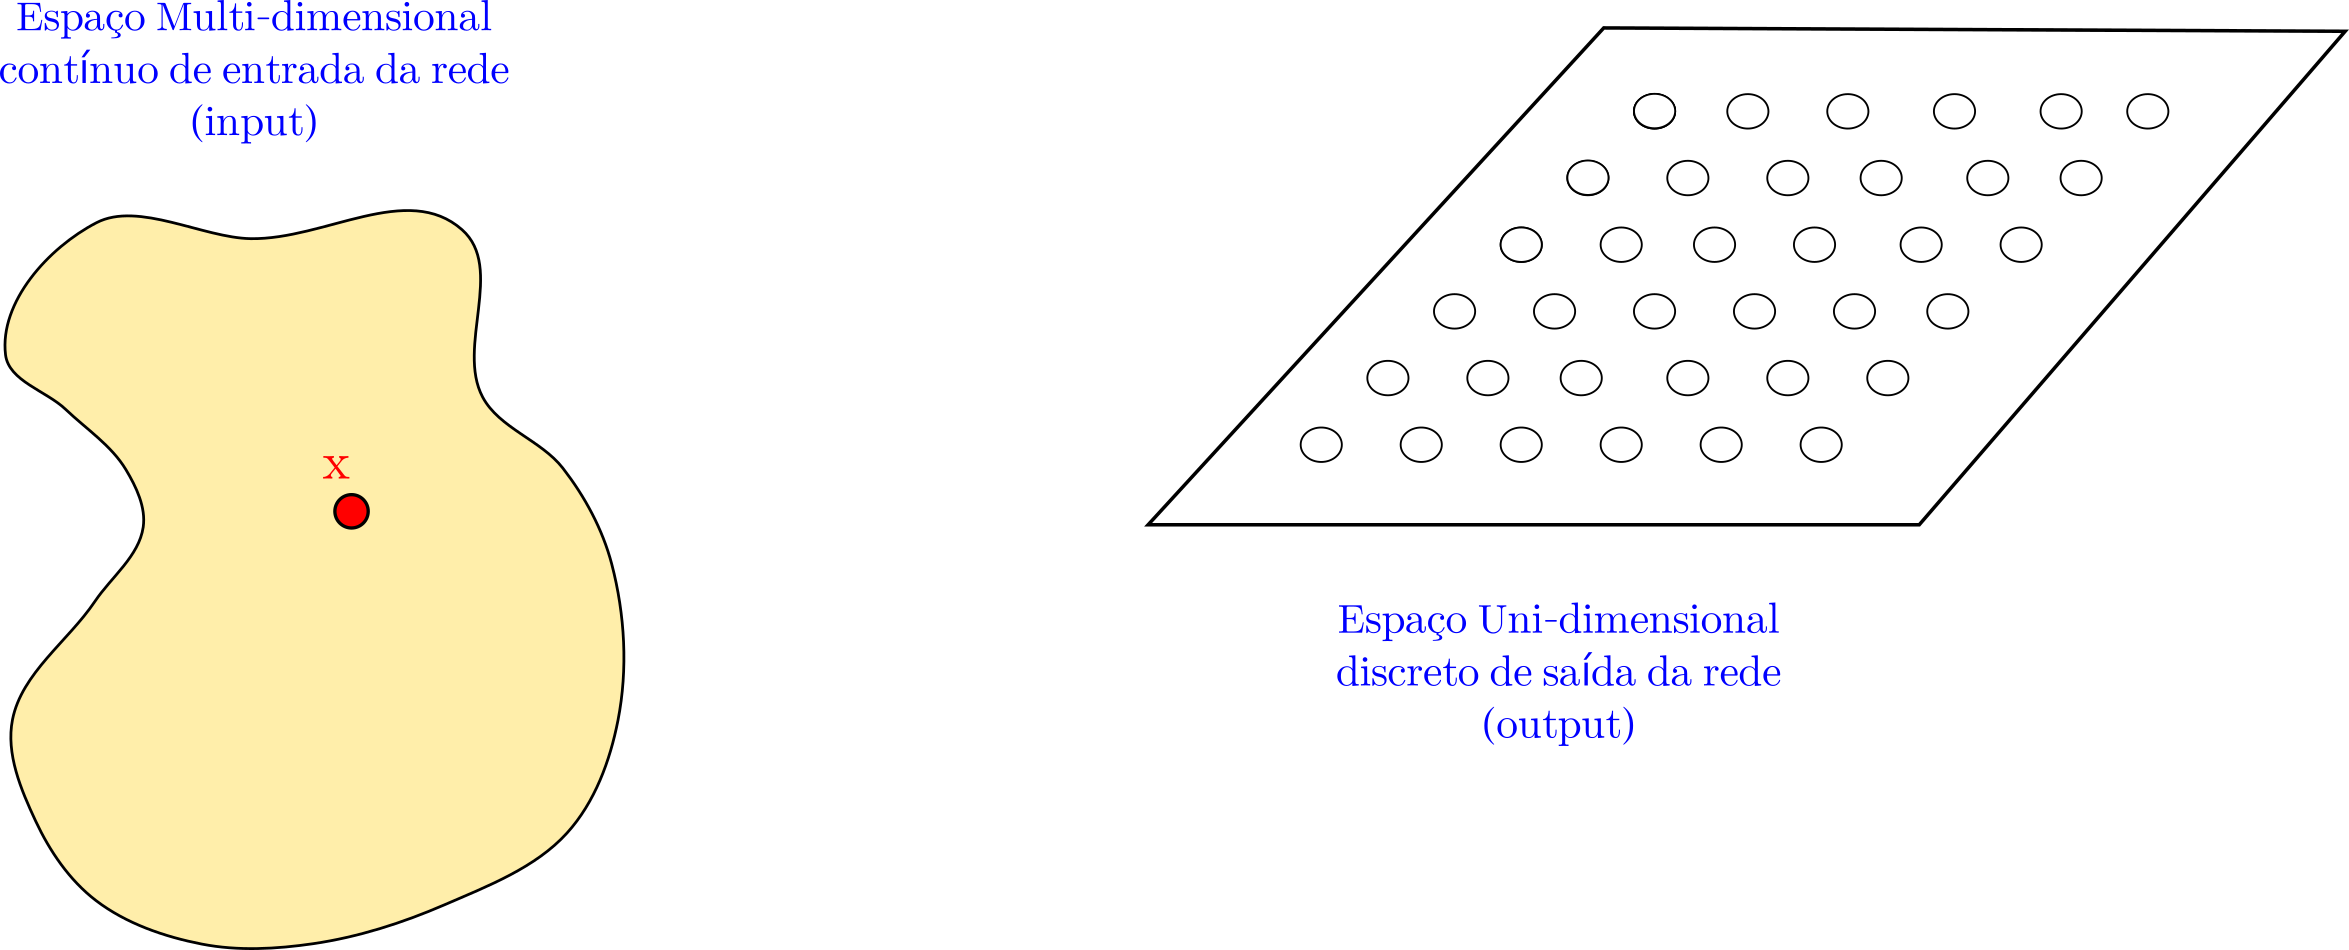
\includegraphics[scale=0.5]{Imagens/IntroKoho3.png} 
\end{frame}

\begin{frame}
 \frametitle{Kohonen - SOM}
 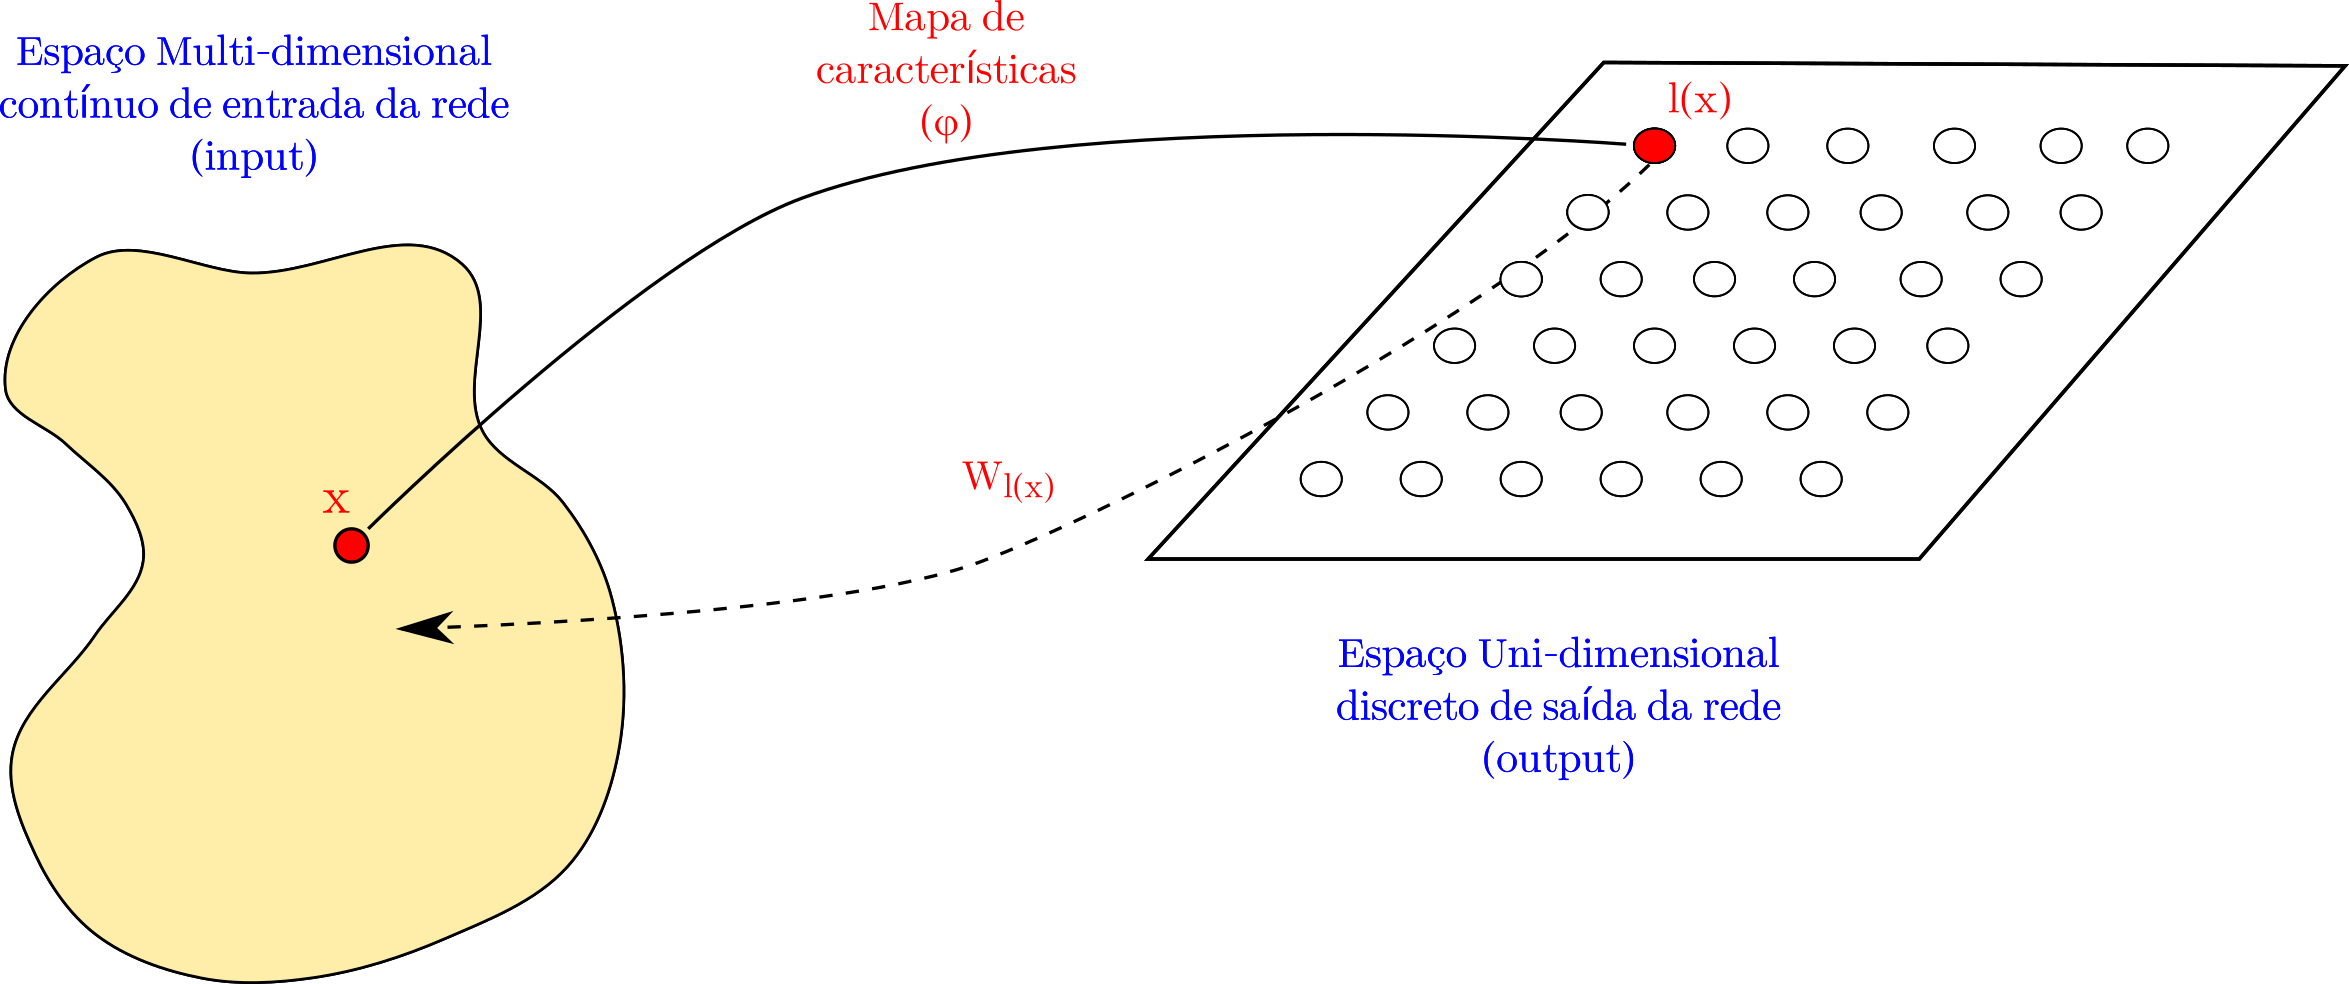
\includegraphics[scale=0.5]{Imagens/IntroKoho4.png} 
\end{frame}

\begin{frame}
	\frametitle{Kohonen - SOM}
	\framesubtitle{Organization}

	\begin{eqnarray}
	\textbf{x}=[x_{1}, x_{2}, x_{3}, ..., x_{m}]^{T} \nonumber
	\end{eqnarray}
	\pause
	\begin{eqnarray}
	\textbf{w}_{j}= [w_{j1}, w_{j2}, w_{j3}, ..., w_{jm}]^{T} \nonumber
	\end{eqnarray}
	\pause
	\begin{eqnarray}
	j=1,2,3,\hdots,l \nonumber
	\end{eqnarray}
\end{frame}

\begin{frame}
    \frametitle{Kohonen - SOM}
    \framesubtitle{Cooperation}
	\begin{eqnarray}
	i(\textbf{x})= argmin_{j}  \parallel \textbf{x} - \textbf{w}_{j} \parallel \nonumber
	\end{eqnarray}
	
	\begin{eqnarray}
	d(t)= \sqrt{\sum^{n}_{i=1}[x(t)-w_{i,j}(t)]^{2}} \hspace{1cm}  (j = {1,..,m}), \nonumber
	\label{eq1}
	\end{eqnarray}
	
	\begin{itemize}
		\centering
		\item[d(t)] distance or identity of a neuron i
	\end{itemize}

\end{frame}



\begin{frame}
 \frametitle{Kohonen - SOM}
 \framesubtitle{Synaptic adaption or Training process}
%Neuron changes the value of the surrounding neurons inside a quartet geometry
%
\begin{equation}
w_{i,j}(t+1)=w_{i,j}(t)+\eta(t)[x(t)-w_{i,j}(t)] \nonumber
\label{eq2}
\end{equation}  

\pause

\begin{itemize}
	\centering
	\item[$w_{i,j}(t+1)$],  updated weight matrix 
	\item[$\eta(t)$], learning rate
\end{itemize}

\begin{equation}
\eta(t)=\eta(0)    ( 1 -  \frac{t}{T}  ) \nonumber
\label{eq3}
\end{equation}  

\begin{itemize}
	\centering
	\item[$T$], number of training cyles
	\pause
	\item[$t$], number of iteractions
	\pause
	\item A iteractive process $t=t+1$ goes on until $t \approx  T$. Once the process ends for one neuron it repeats it self for the surrounding neighbors \citep{YANG2009,Yan2014}.
\end{itemize}

%Where $T$ is the number of training cyles and $t$ is the number of iteractions. A iteractive process $t=t+1$ goes on until $t \approx  T$. Once the process ends for one neuron it repeats it self for the surrounding neighbors.

\end{frame}


\begin{frame}
\frametitle{The geometry}

\begin{figure}[H]
\flushleft
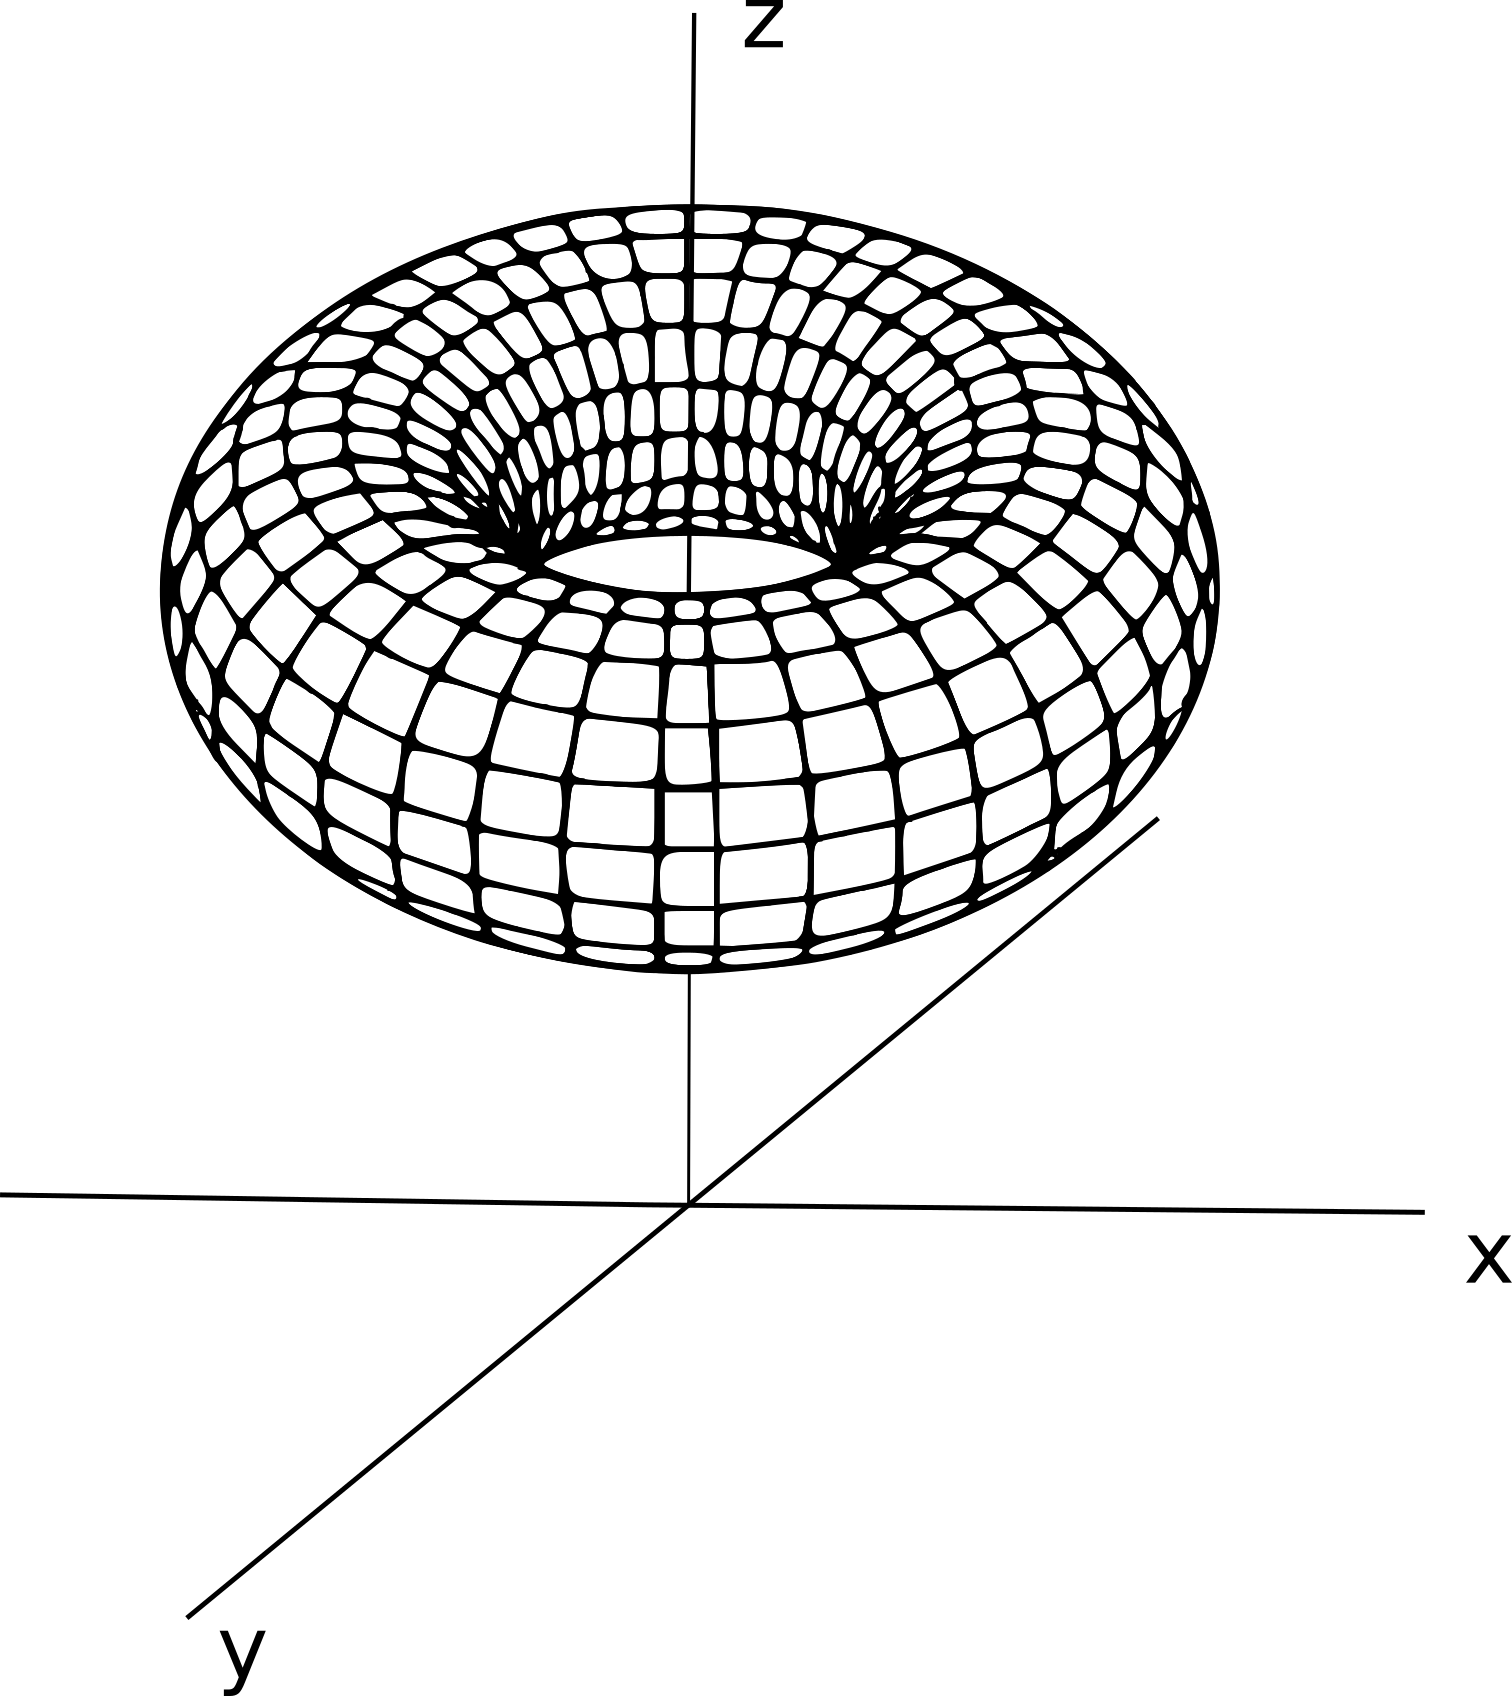
\includegraphics[scale=0.2]{Imagens/toro.png}
\label{toro}
\end{figure}
\begin{figure}
\flushright
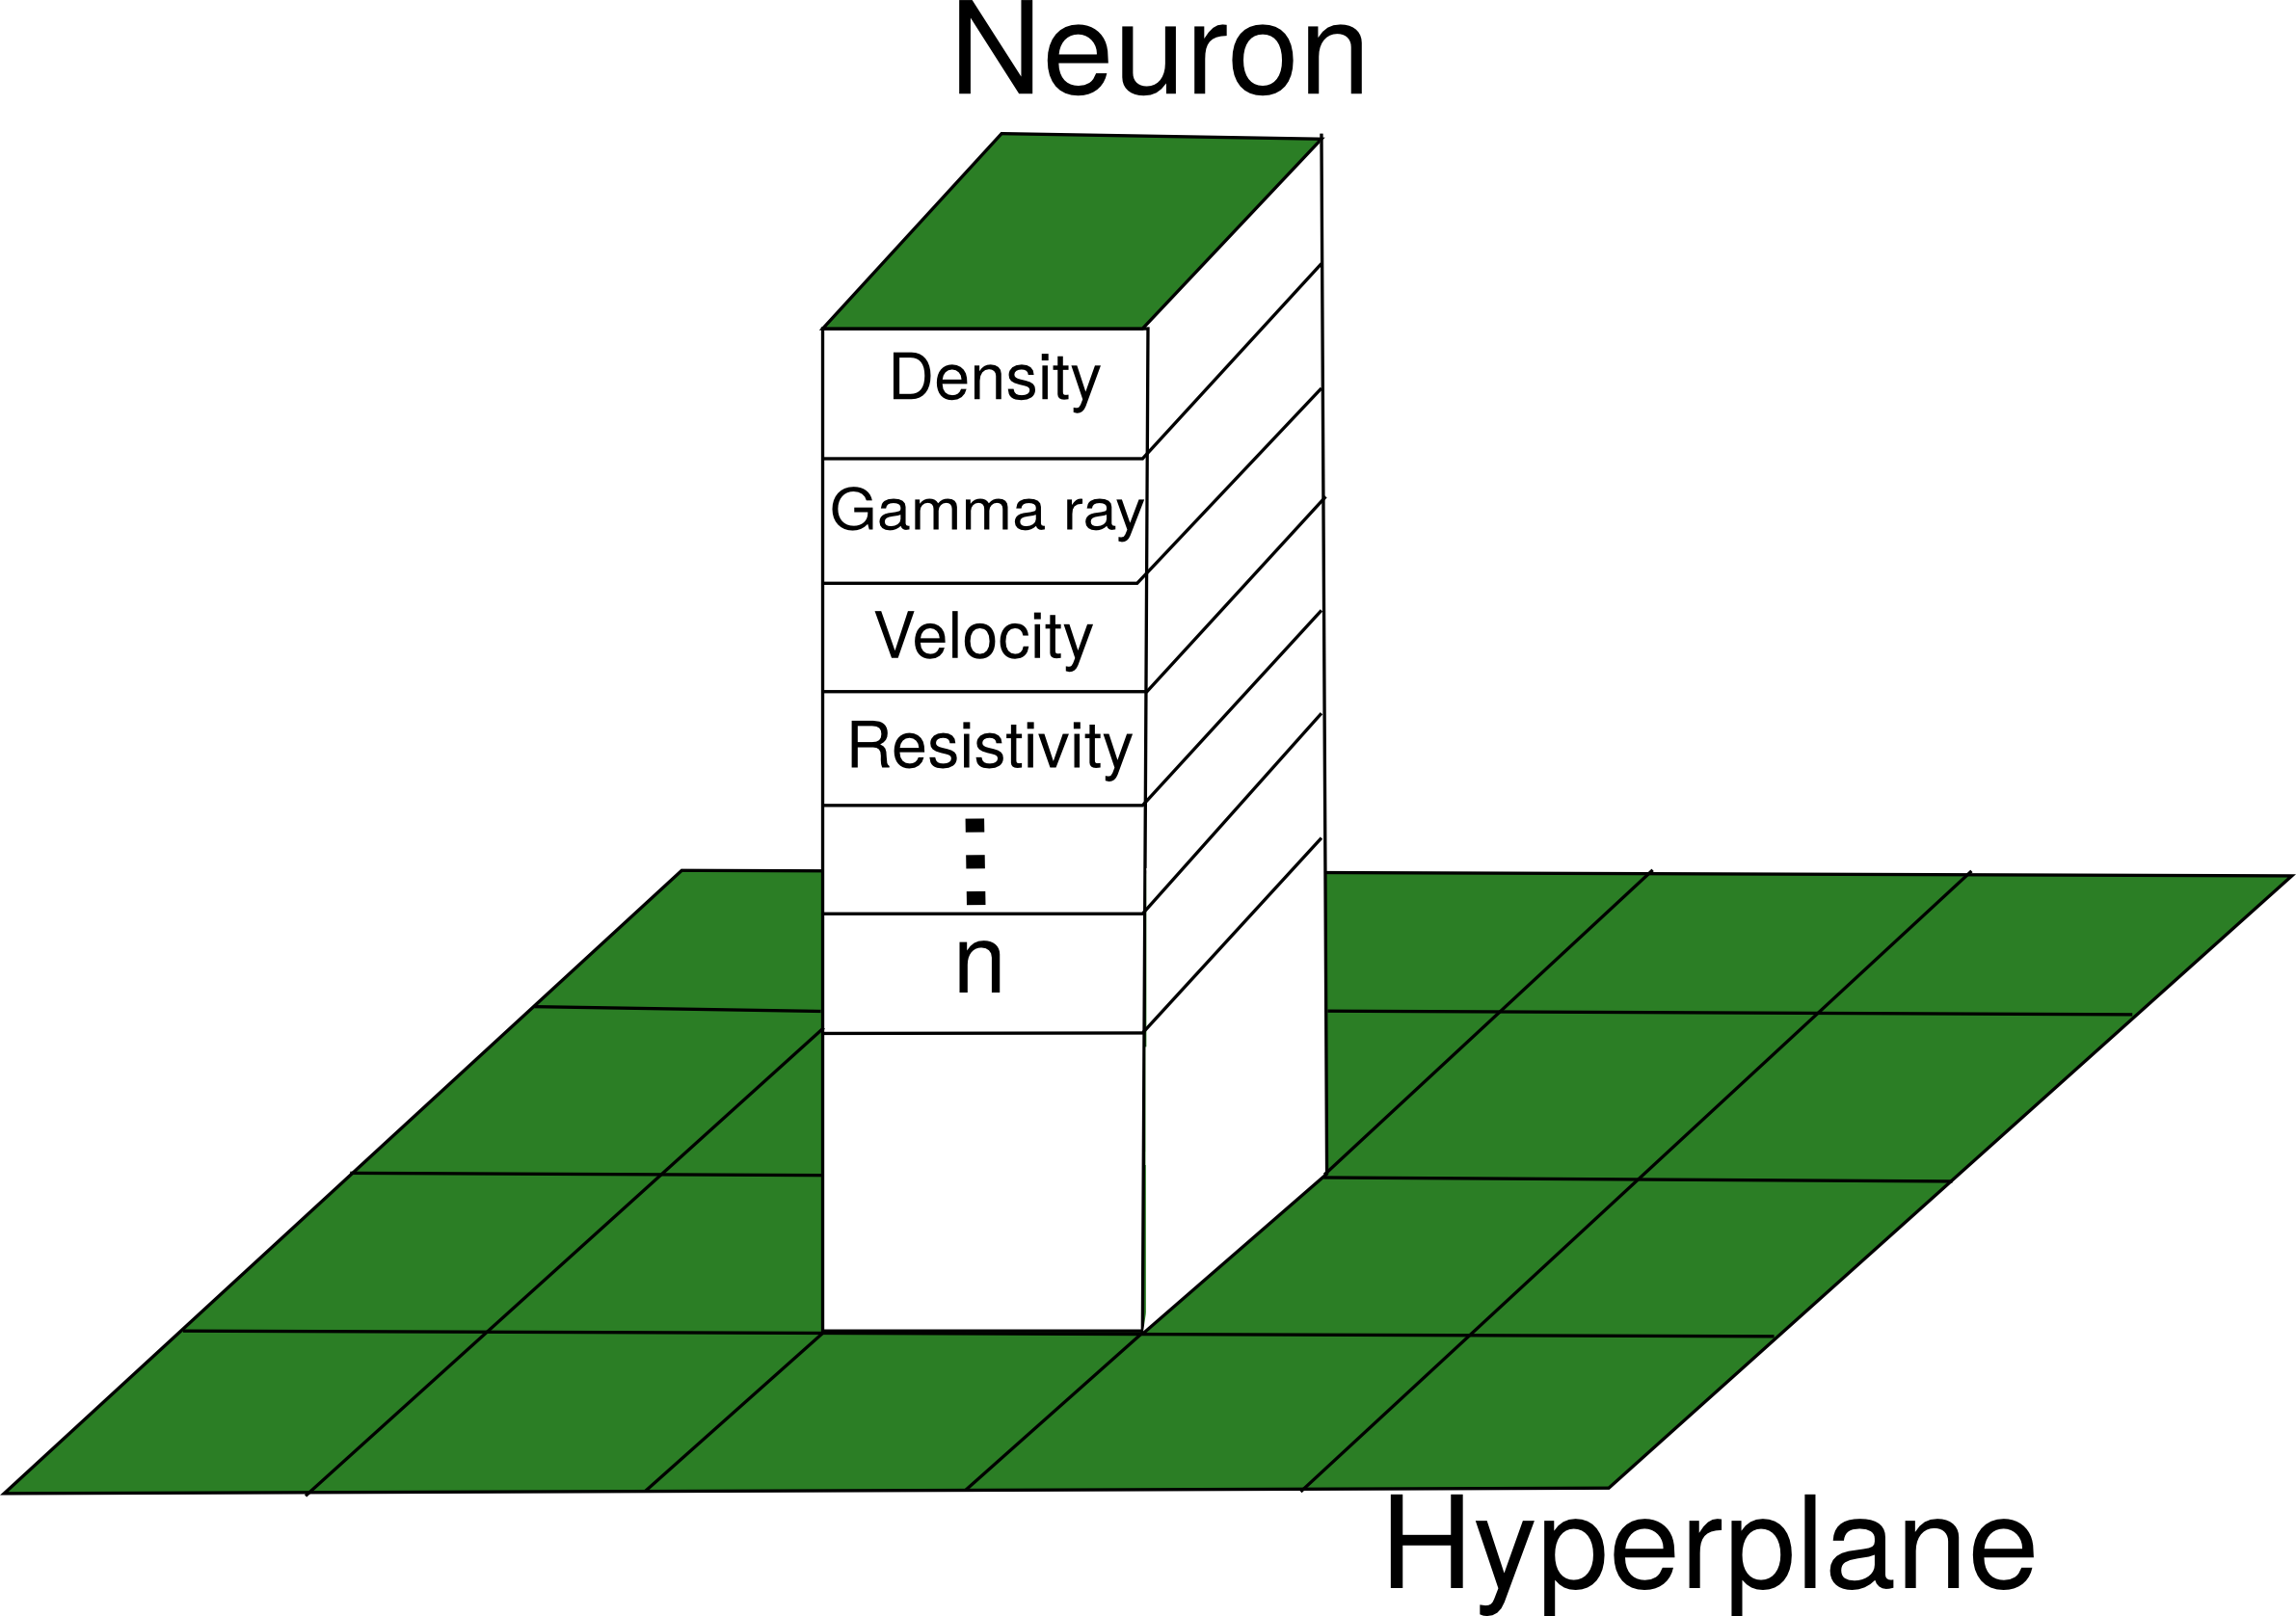
\includegraphics[scale=0.33]{Imagens/hiperplano.png}
\label{hiperplano}
\end{figure}
\end{frame}


\begin{frame}
\frametitle{A hyperplane with $400$ neurons}
\centering
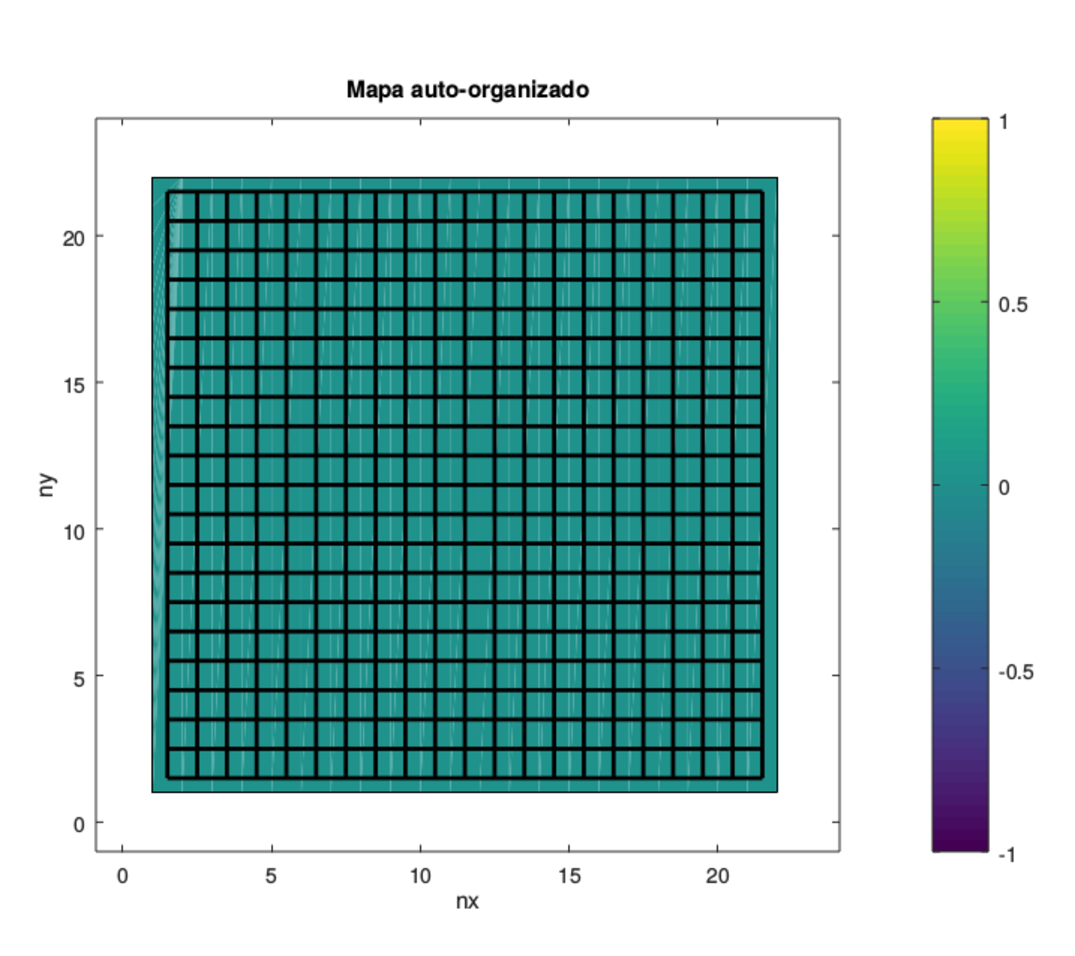
\includegraphics[scale=0.47]{Imagens/SOM1_2d.pdf} 
\end{frame}

\begin{frame}
\frametitle{A hyperplane with $400$ neurons}
\centering
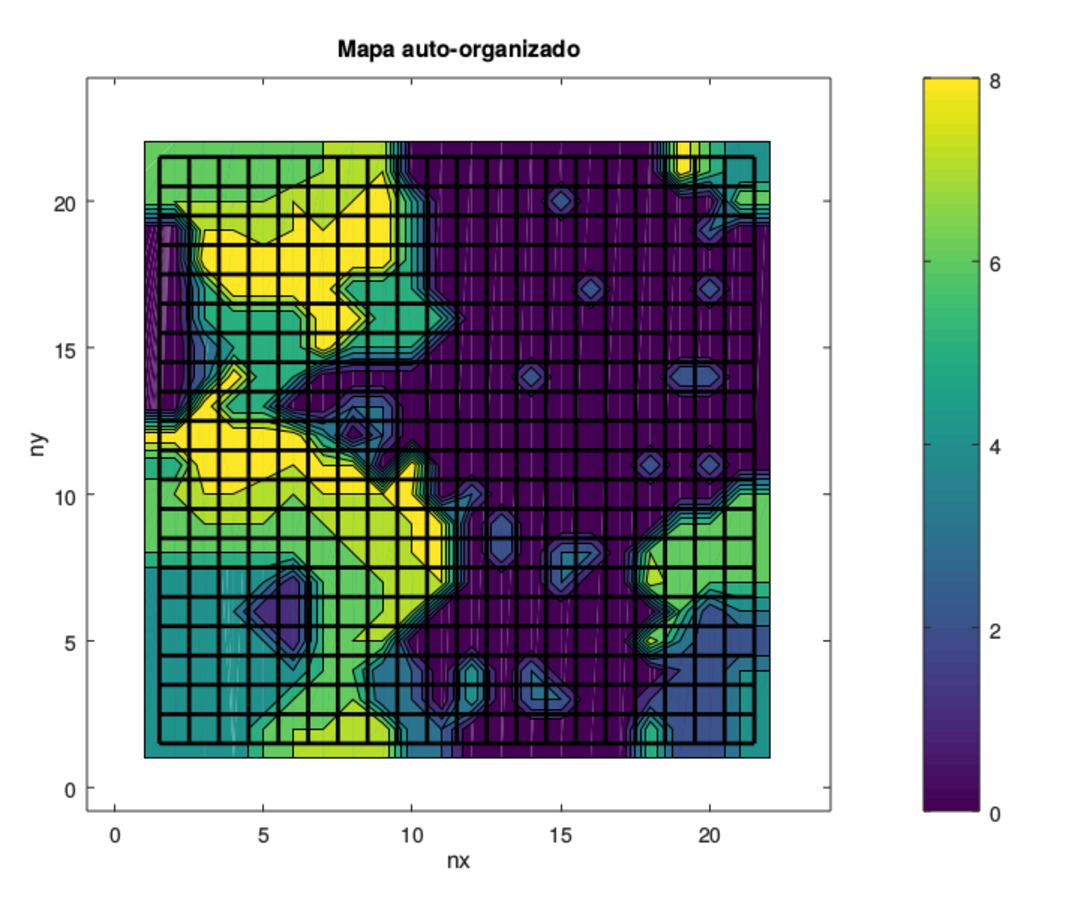
\includegraphics[scale=0.47]{Imagens/SOM5_2d.pdf} 
\end{frame}

\begin{frame}
\frametitle{A hyperplane with $400$ neurons}
\centering
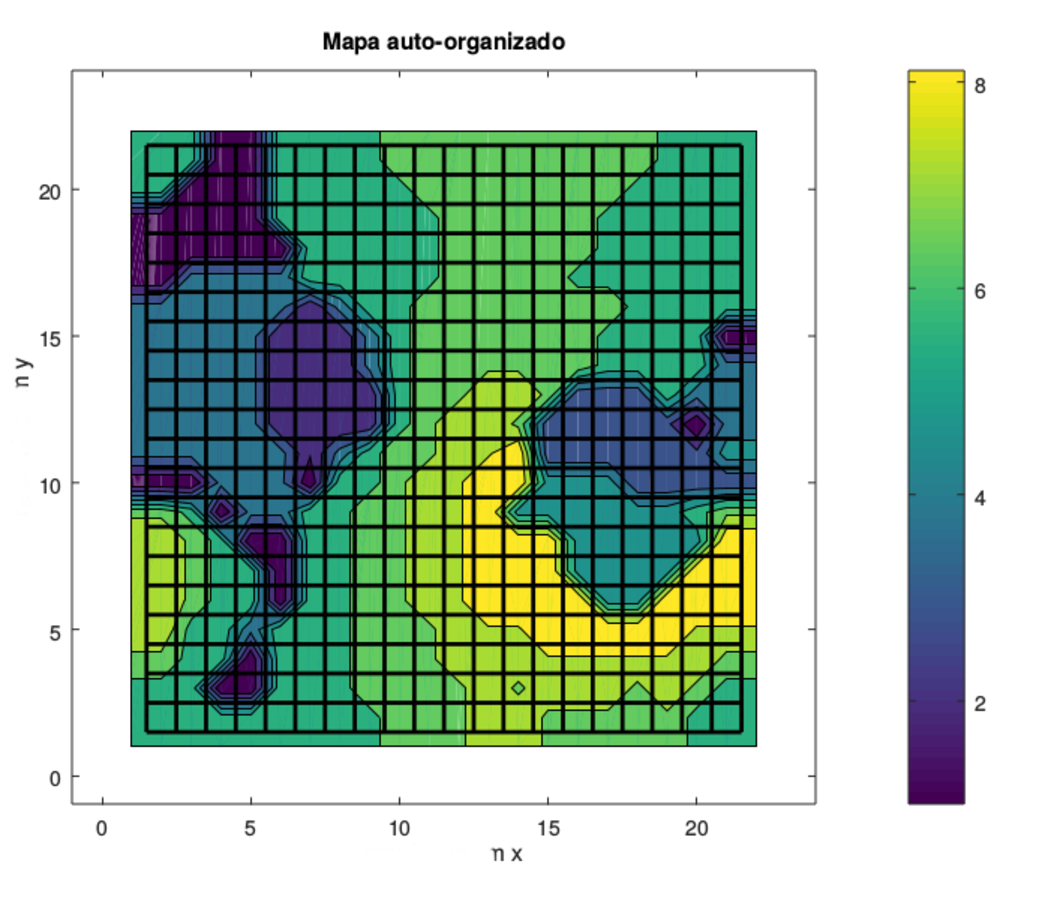
\includegraphics[scale=0.47]{Imagens/SOM100_2d.pdf} 
\end{frame}

\begin{frame}
\frametitle{A hyperplane with $400$ neurons}
\centering
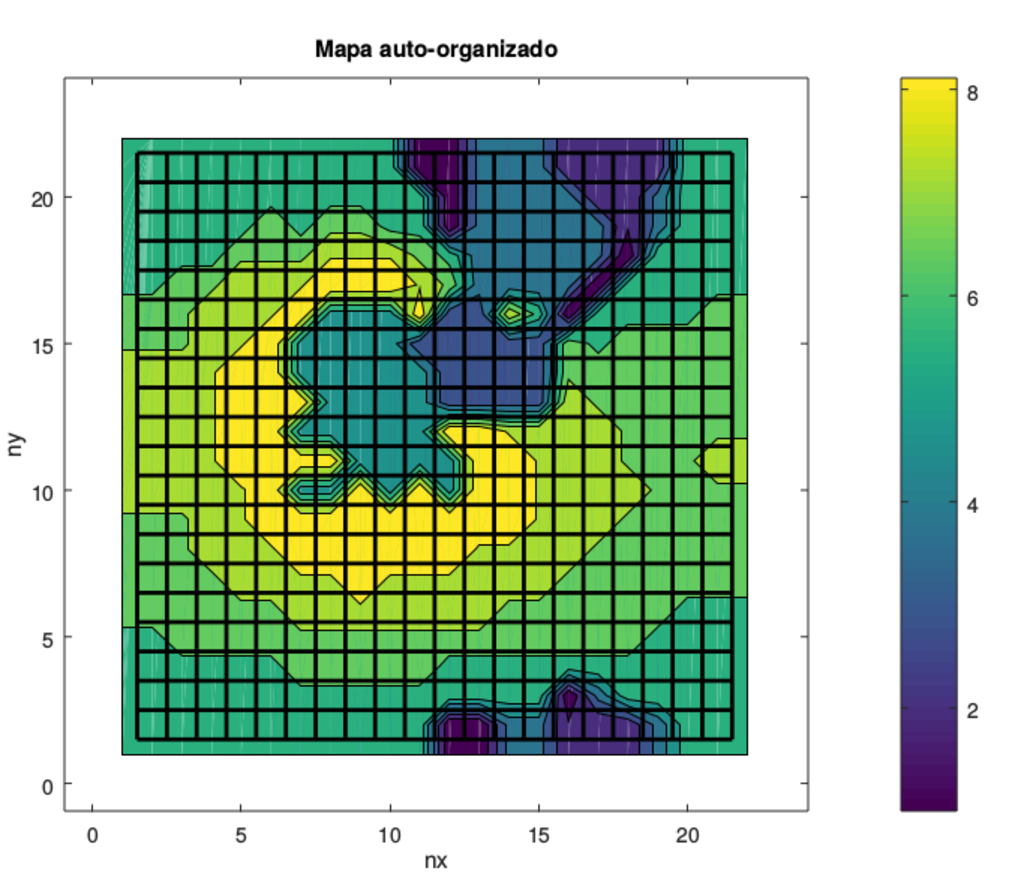
\includegraphics[scale=0.47]{Imagens/SOM1000_2d.pdf} 
\end{frame}


\begin{frame}
	\frametitle{A hyperplane with $400$ neurons}
	\begin{table}[H]
		\centering
		\begin{tabular}{c|c}
			
			Lithology                   & Normalization \\ % Note a separação de col. e a quebra de linhas
			\hline                                                             % para uma linha horizontal
			Shale 2                 &  1\\
			Dolomite  		            &  2 \\
			Diabase    	            &  3 \\
			Conglomerate          &  4 \\
			Conglomerate 80\% &  5  \\
			Conglomerate 60\%&  6 \\
			Conglomerate 40\%&  7\\
			Conglomerate 20\%&  8 \\
			Crystalline Basement          &  9 \\
			% não é preciso quebrar a última linha
			
		\end{tabular}
		\label{codigos}
		%\caption{Tabela de referência para conversão do padrão numérico em litologia.}
	\end{table}
\end{frame}

\section{Results}

\begin{frame}
\frametitle{Results}
\framesubtitle{Classifications C1}
	\begin{figure}[H]
		\centering
		 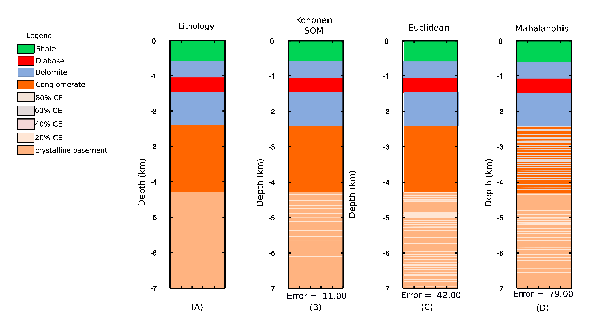
\includegraphics[scale=0.35]{Imagens/IDC1020118.eps}
	%	\caption{Comparison between the classifiers and SOM for C1 well data. }
		\label{C1}
	\end{figure}
\end{frame}

\begin{frame}
\frametitle{Results}
\framesubtitle{Classifications C2}
	\begin{figure}[H]
		\centering
		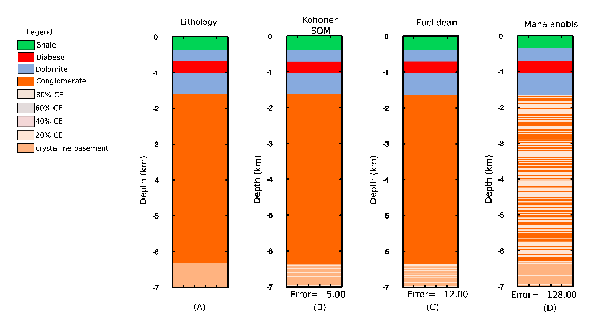
\includegraphics[scale=0.35]{Imagens/IDC2020118.eps}
	%	\caption{Comparison between the classifiers and SOM for C2 well data. }
		\label{C2}
	\end{figure}
\end{frame}

\section{Conclusions}

\begin{frame}
	\frametitle{Conclusions}
	\begin{itemize}
		\item SOM algorithm overperformed the euclidean and mahalanobis classifiers with an error of $0.71\%$
		\pause
		\item The complex distribution of features on the space of properties led to an increase of errors on classifiers of $18.28\%$ (mahalanobis) and $1.74\%$ (euclidean)
		\pause
		\item Classifiers can not perform classification of bell patterns in well data. 
		\pause
		\item Box patterns could be solved with euclidean classifier but not in mahalanobis
		\pause
		\item Kohonen - SOM showed the bests results concerning classification of mixture of rocks or the bell pattern
	\end{itemize}
\end{frame}


%\section{References}

\begin{frame}[allowframebreaks]
\frametitle{References}
%\beamertemplatetextbibitems
\tiny
\bibliographystyle{apalike}
\bibliography{references}
\end{frame}

\begin{frame}
\flushbottom
\setlength{\parskip}{-1ex plus 1ex }
\setlength{\parindent}{-15pt}
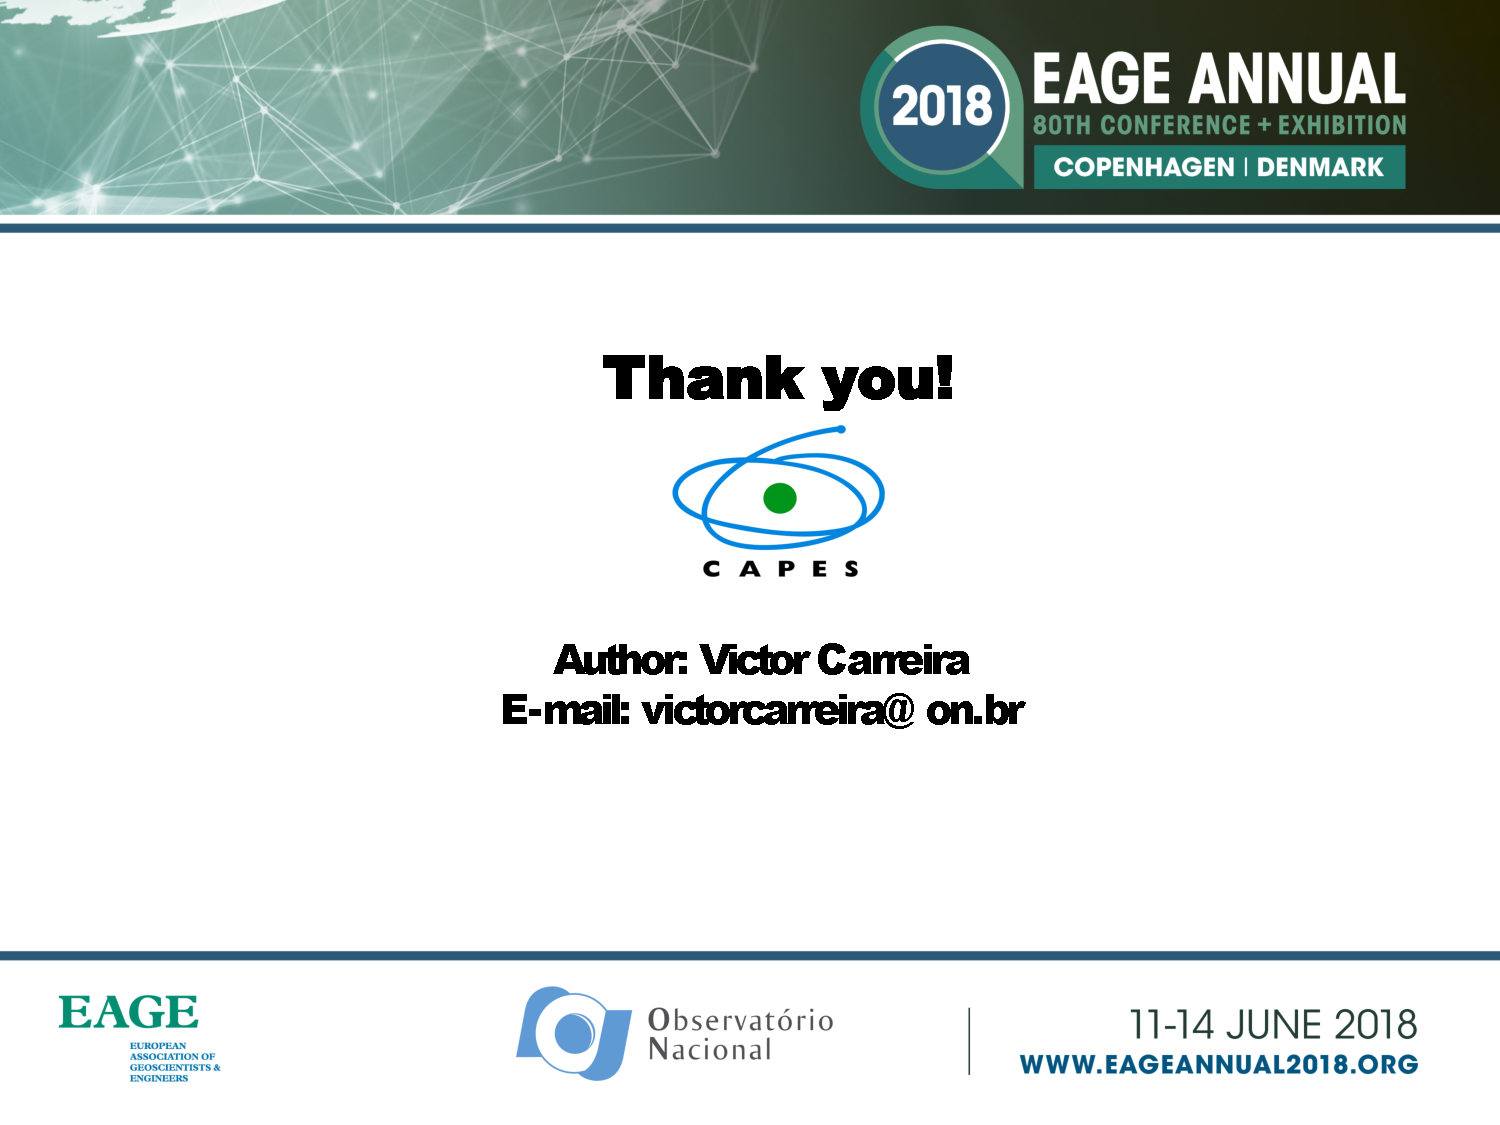
\includegraphics[width=13cm,height=10cm]{Imagens/end.pdf}
\end{frame}

\end{document}